% Created 2022-05-31 Tue 23:45
% Intended LaTeX compiler: pdflatex
\documentclass[12pt]{article}

%%%% settings when exporting code %%%% 

\usepackage{listings}
\lstdefinestyle{code-small}{
backgroundcolor=\color{white}, % background color for the code block
basicstyle=\ttfamily\small, % font used to display the code
commentstyle=\color[rgb]{0.5,0,0.5}, % color used to display comments in the code
keywordstyle=\color{black}, % color used to highlight certain words in the code
numberstyle=\ttfamily\tiny\color{gray}, % color used to display the line numbers
rulecolor=\color{black}, % color of the frame
stringstyle=\color[rgb]{0,.5,0},  % color used to display strings in the code
breakatwhitespace=false, % sets if automatic breaks should only happen at whitespace
breaklines=true, % sets automatic line breaking
columns=fullflexible,
frame=single, % adds a frame around the code (non,leftline,topline,bottomline,lines,single,shadowbox)
keepspaces=true, % % keeps spaces in text, useful for keeping indentation of code
literate={~}{$\sim$}{1}, % symbol properly display via latex
numbers=none, % where to put the line-numbers; possible values are (none, left, right)
numbersep=10pt, % how far the line-numbers are from the code
showspaces=false,
showstringspaces=false,
stepnumber=1, % the step between two line-numbers. If it's 1, each line will be numbered
tabsize=1,
xleftmargin=0cm,
emph={anova,apply,class,coef,colnames,colNames,colSums,dim,dcast,for,ggplot,head,if,ifelse,is.na,lapply,list.files,library,logLik,melt,plot,require,rowSums,sapply,setcolorder,setkey,str,summary,tapply},
aboveskip = \medskipamount, % define the space above displayed listings.
belowskip = \medskipamount, % define the space above displayed listings.
lineskip = 0pt} % specifies additional space between lines in listings
\lstset{style=code-small}
%%%% packages %%%%%

\usepackage[utf8]{inputenc}
\usepackage[T1]{fontenc}
\usepackage{lmodern}
\usepackage{textcomp}
\usepackage{color}
\usepackage{graphicx}
\usepackage{grffile}
\usepackage{wrapfig}
\usepackage{rotating}
\usepackage{longtable}
\usepackage{multirow}
\usepackage{multicol}
\usepackage{changes}
\usepackage{pdflscape}
\usepackage{geometry}
\usepackage[normalem]{ulem}
\usepackage{amssymb}
\usepackage{amsmath}
\usepackage{amsfonts}
\usepackage{dsfont}
\usepackage{array}
\usepackage{ifthen}
\usepackage{hyperref}
\usepackage{natbib}
\RequirePackage{setspace} % to modify the space between lines - incompatible with footnote in beamer
\renewcommand{\baselinestretch}{1.1}
\geometry{a4paper, left=10mm, right=10mm, top=10mm}
\usepackage{titlesec}
\usepackage{etoolbox}

\makeatletter
\patchcmd{\ttlh@hang}{\parindent\z@}{\parindent\z@\leavevmode}{}{}
\patchcmd{\ttlh@hang}{\noindent}{}{}{}
\makeatother
\RequirePackage{colortbl} % arrayrulecolor to mix colors
\definecolor{myorange}{rgb}{1,0.2,0}
\definecolor{mypurple}{rgb}{0.7,0,8}
\definecolor{mycyan}{rgb}{0,0.6,0.6}
\newcommand{\lightblue}{blue!50!white}
\newcommand{\darkblue}{blue!80!black}
\newcommand{\darkgreen}{green!50!black}
\newcommand{\darkred}{red!50!black}
\definecolor{gray}{gray}{0.5}
\hypersetup{
citecolor=[rgb]{0,0.5,0},
urlcolor=[rgb]{0,0,0.5},
linkcolor=[rgb]{0,0,0.5},
}
\newenvironment{note}{\small \color{gray}\fontfamily{lmtt}\selectfont}{\par}
\newenvironment{activity}{\color{orange}\fontfamily{qzc}\selectfont}{\par}
\RequirePackage{pifont}
\RequirePackage{relsize}
\newcommand{\Cross}{{\raisebox{-0.5ex}%
{\relsize{1.5}\ding{56}}}\hspace{1pt} }
\newcommand{\Valid}{{\raisebox{-0.5ex}%
{\relsize{1.5}\ding{52}}}\hspace{1pt} }
\newcommand{\CrossR}{ \textcolor{red}{\Cross} }
\newcommand{\ValidV}{ \textcolor{green}{\Valid} }
\usepackage{stackengine}
\usepackage{scalerel}
\newcommand\Warning[1][3ex]{%
\renewcommand\stacktype{L}%
\scaleto{\stackon[1.3pt]{\color{red}$\triangle$}{\tiny\bfseries !}}{#1}%
\xspace
}
\newcommand\Rlogo{\textbf{\textsf{R}}\xspace} %
\RequirePackage{fancyvrb}
\DefineVerbatimEnvironment{verbatim}{Verbatim}{fontsize=\small,formatcom = {\color[rgb]{0.5,0,0}}}
\RequirePackage{enumitem} % better than enumerate
\RequirePackage{epstopdf} % to be able to convert .eps to .pdf image files
\RequirePackage{capt-of} %
\RequirePackage{caption} % newlines in graphics
\RequirePackage{tikz-cd} % graph
\RequirePackage{booktabs} % for nice lines in table (e.g. toprule, bottomrule, midrule, cmidrule)
\RequirePackage{amsmath}
\RequirePackage{algorithm}
\RequirePackage[noend]{algpseudocode}
\RequirePackage{dsfont}
\RequirePackage{amsmath,stmaryrd,graphicx}
\RequirePackage{prodint} % product integral symbol (\PRODI)
\usepackage{ifthen}
\usepackage{xifthen}
\usepackage{xargs}
\usepackage{xspace}
\newcommand\defOperator[7]{%
\ifthenelse{\isempty{#2}}{
\ifthenelse{\isempty{#1}}{#7{#3}#4}{#7{#3}#4 \left#5 #1 \right#6}
}{
\ifthenelse{\isempty{#1}}{#7{#3}#4_{#2}}{#7{#3}#4_{#1}\left#5 #2 \right#6}
}
}
\newcommand\defUOperator[5]{%
\ifthenelse{\isempty{#1}}{
#5\left#3 #2 \right#4
}{
\ifthenelse{\isempty{#2}}{\underset{#1}{\operatornamewithlimits{#5}}}{
\underset{#1}{\operatornamewithlimits{#5}}\left#3 #2 \right#4}
}
}
\newcommand{\defBoldVar}[2]{
\ifthenelse{\equal{#2}{T}}{\boldsymbol{#1}}{\mathbf{#1}}
}
\newcommandx\Esp[2][1=,2=]{\defOperator{#1}{#2}{E}{}{\lbrack}{\rbrack}{\mathbb}}
\newcommandx\Prob[2][1=,2=]{\defOperator{#1}{#2}{P}{}{\lbrack}{\rbrack}{\mathbb}}
\newcommandx\Qrob[2][1=,2=]{\defOperator{#1}{#2}{Q}{}{\lbrack}{\rbrack}{\mathbb}}
\newcommandx\Var[2][1=,2=]{\defOperator{#1}{#2}{V}{ar}{\lbrack}{\rbrack}{\mathbb}}
\newcommandx\Cov[2][1=,2=]{\defOperator{#1}{#2}{C}{ov}{\lbrack}{\rbrack}{\mathbb}}
\newcommandx\Binom[2][1=,2=]{\defOperator{#1}{#2}{B}{}{(}{)}{\mathcal}}
\newcommandx\Gaus[2][1=,2=]{\defOperator{#1}{#2}{N}{}{(}{)}{\mathcal}}
\newcommandx\Wishart[2][1=,2=]{\defOperator{#1}{#2}{W}{ishart}{(}{)}{\mathcal}}
\newcommandx\Likelihood[2][1=,2=]{\defOperator{#1}{#2}{L}{}{(}{)}{\mathcal}}
\newcommandx\logLikelihood[2][1=,2=]{\defOperator{#1}{#2}{\ell}{}{(}{)}{}}
\newcommandx\Information[2][1=,2=]{\defOperator{#1}{#2}{I}{}{(}{)}{\mathcal}}
\newcommandx\Hessian[2][1=,2=]{\defOperator{#1}{#2}{H}{}{(}{)}{\mathcal}}
\newcommandx\Score[2][1=,2=]{\defOperator{#1}{#2}{S}{}{(}{)}{\mathcal}}
\newcommandx\Vois[2][1=,2=]{\defOperator{#1}{#2}{V}{}{(}{)}{\mathcal}}
\newcommandx\IF[2][1=,2=]{\defOperator{#1}{#2}{IF}{}{(}{)}{\mathcal}}
\newcommandx\Ind[1][1=]{\defOperator{}{#1}{1}{}{(}{)}{\mathds}}
\newcommandx\Max[2][1=,2=]{\defUOperator{#1}{#2}{(}{)}{min}}
\newcommandx\Min[2][1=,2=]{\defUOperator{#1}{#2}{(}{)}{max}}
\newcommandx\argMax[2][1=,2=]{\defUOperator{#1}{#2}{(}{)}{argmax}}
\newcommandx\argMin[2][1=,2=]{\defUOperator{#1}{#2}{(}{)}{argmin}}
\newcommandx\cvD[2][1=D,2=n \rightarrow \infty]{\xrightarrow[#2]{#1}}
\newcommandx\Hypothesis[2][1=,2=]{
\ifthenelse{\isempty{#1}}{
\mathcal{H}
}{
\ifthenelse{\isempty{#2}}{
\mathcal{H}_{#1}
}{
\mathcal{H}^{(#2)}_{#1}
}
}
}
\newcommandx\dpartial[4][1=,2=,3=,4=\partial]{
\ifthenelse{\isempty{#3}}{
\frac{#4 #1}{#4 #2}
}{
\left.\frac{#4 #1}{#4 #2}\right\rvert_{#3}
}
}
\newcommandx\dTpartial[3][1=,2=,3=]{\dpartial[#1][#2][#3][d]}
\newcommandx\ddpartial[3][1=,2=,3=]{
\ifthenelse{\isempty{#3}}{
\frac{\partial^{2} #1}{\partial #2^2}
}{
\frac{\partial^2 #1}{\partial #2\partial #3}
}
}
\newcommand\Real{\mathbb{R}}
\newcommand\Rational{\mathbb{Q}}
\newcommand\Natural{\mathbb{N}}
\newcommand\trans[1]{{#1}^\intercal}%\newcommand\trans[1]{{\vphantom{#1}}^\top{#1}}
\newcommand{\independent}{\mathrel{\text{\scalebox{1.5}{$\perp\mkern-10mu\perp$}}}}
\newcommand\half{\frac{1}{2}}
\newcommand\normMax[1]{\left|\left|#1\right|\right|_{max}}
\newcommand\normTwo[1]{\left|\left|#1\right|\right|_{2}}
\newcommand\Veta{\boldsymbol{\eta}}
\newcommand{\Model}{\mathcal{M}}
\newcommand{\ModelHat}{\widehat{\mathcal{M}}}
\newcommand{\param}{\Theta}
\newcommand{\paramHat}{\widehat{\param}}
\newcommand{\paramCon}{\widetilde{\param}}
\newcommand{\Vparam}{\boldsymbol{\param}}
\newcommand{\VparamT}{\Vparam_0}
\newcommand{\VparamHat}{\boldsymbol{\paramHat}}
\newcommand{\VparamCon}{\boldsymbol{\paramCon}}
\newcommand{\X}{X}
\newcommand{\x}{x}
\newcommand{\VX}{\boldsymbol{X}}
\newcommand{\Vx}{\boldsymbol{x}}
\newcommand{\Y}{Y}
\newcommand{\y}{y}
\newcommand{\VY}{\boldsymbol{Y}}
\newcommand{\Vy}{\boldsymbol{y}}
\newcommand{\Vvarepsilon}{\boldsymbol{\varepsilon}}
\author{Brice Ozenne}
\date{\today}
\title{Overview of the package LMMstar}
\hypersetup{
 colorlinks=true,
 pdfauthor={Brice Ozenne},
 pdftitle={Overview of the package LMMstar},
 pdfkeywords={},
 pdfsubject={},
 pdfcreator={Emacs 26.3 (Org mode 9.4.6)},
 pdflang={English}
 }
\begin{document}

\maketitle
This vignette describes the main functionalities of the \textbf{LMMstar}
package. This package implements specific types of linear mixed
models, mainly useful when having repeated observations over a
discrete variable (e.g. time, brain region, \ldots{}). Key assumptions are
that at the cluster level, observation are independent and that the
mean and variance are independent (conditionally on covariates). In
particular, in large samples the residuals do not have to be normally
distributed.

\bigskip

The user interface of the \textbf{LMMstar} package is made of the following functions:
\begin{itemize}
\item the function \texttt{lmm} is the main function of the package which fits
linear mixed models. The user can interact with \emph{lmm} objects using:
\begin{itemize}
\item \texttt{anova} to test linear combinations of coefficients (Wald test
or Likelihood ratio tests). \newline The output be combined via \texttt{rbind}.
\item \texttt{coef} to extract the estimates.
\item \texttt{confint} to extract the estimates with their confidence intervals.
\item \texttt{dummy.coef} to extract the estimated (marginal) mean for each combination of categorical covariate.
\item \texttt{estimate} to test non-linear combinations of coefficients (Wald test via a first order delta method).
\item \texttt{levels} to extract the reference level for the mean structure.
(i.e. what \texttt{(Intercept)} refers to in presence of categorical.
covariates).
\item \texttt{logLik} to output the log-likelihood of the estimated model.
\item \texttt{model.tables} to extract the estimates, standard errors, p-value, and confidence intervals.
\item \texttt{plot} to obtain a diagnostic plots, partial residual plots, or a graphical display of the fitted values.
\item \texttt{predict} to compute the conditional mean for new observations.
\item \texttt{residuals} to extract the observed residuals of the fitted model.
\item \texttt{sigma} to extract the modeled residual variance covariance matrix.
\item \texttt{summary} to obtain a summary of the input, model fit, and estimated values.
\end{itemize}
\item the \texttt{mlmm} function to fit (distinct) linear mixed models on
different outcome, and gather the estimated coefficients.
\item the \texttt{summarize} function to compute summary statistics stratified on a categorical variable.
\item the \texttt{partialCor} function to compute partial correlation between two variables.
\item the \texttt{sampleRem} function to simulate longitudinal data.
\item the \texttt{LMMstar.options} function enables the user to display the
default values used in the \textbf{LMMstar} package. The function
can also change the default values to better match the user needs.
\end{itemize}

\bigskip

Before going further we need to load the \textbf{LMMstar} package in the R
session:
\lstset{language=r,label= ,caption= ,captionpos=b,numbers=none}
\begin{lstlisting}
library(LMMstar)
\end{lstlisting}

To illustrate the functionalities of the package, we will use the
gastricbypass dataset:
\lstset{language=r,label= ,caption= ,captionpos=b,numbers=none}
\begin{lstlisting}
data(gastricbypassL, package = "LMMstar")
head(gastricbypassL)
\end{lstlisting}

\begin{verbatim}
  id visit          time weight glucagonAUC
1  1     1 3monthsBefore  127.2     5032.50
2  2     1 3monthsBefore  165.2    12142.50
3  3     1 3monthsBefore  109.7    10321.35
4  4     1 3monthsBefore  146.2     6693.00
5  5     1 3monthsBefore  113.1     7090.50
6  6     1 3monthsBefore  158.8    10386.00
\end{verbatim}


See \texttt{?gastricbypassL} for a presentation of the database. We will use a shorter version of the time variable:
\lstset{language=r,label= ,caption= ,captionpos=b,numbers=none}
\begin{lstlisting}
gastricbypassL$time <- factor(gastricbypassL$time,
			      levels = c("3monthsBefore", "1weekBefore",
					 "1weekAfter", "3monthsAfter" ),
			      labels = c("B3m","B1w","A1w","A3m"))
gastricbypassL$visit <- as.numeric(gastricbypassL$time) ## convert to numeric
gastricbypassL$baseline <- gastricbypassL$visit<=2
\end{lstlisting}
rescale the glucagon values
\lstset{language=r,label= ,caption= ,captionpos=b,numbers=none}
\begin{lstlisting}
gastricbypassL$glucagon <- as.double(scale(gastricbypassL$glucagonAUC))+5
\end{lstlisting}

and add a group variable:
\lstset{language=r,label= ,caption= ,captionpos=b,numbers=none}
\begin{lstlisting}
gastricbypassL$group <- as.numeric(gastricbypassL$id)%%2
\end{lstlisting}

\bigskip

\uline{Note:} the \textbf{LMMstar} package is under active development. Newer
package versions may include additional functionalities and fix
previous bugs. The version of the package that is being used is:
\lstset{language=r,label= ,caption= ,captionpos=b,numbers=none}
\begin{lstlisting}
utils::packageVersion("LMMstar")
\end{lstlisting}

\begin{verbatim}
[1] ‘0.7.1’
\end{verbatim}


When estimating model coefficients, we will use the internal
optimization routine of the \textbf{LMMstar} package (instead of relying on
the \texttt{nlme::gls} function, which is the default option):
\lstset{language=r,label= ,caption= ,captionpos=b,numbers=none}
\begin{lstlisting}
LMMstar.options(optimizer = "FS")
\end{lstlisting}

\clearpage

\section{Descriptive statistics}
\label{sec:org05d6ac4}
Mean, standard deviation, and other summary statistic can be computed
with respect to a categorical variable (typically time) using the
\texttt{summarize} function:
\lstset{language=r,label= ,caption= ,captionpos=b,numbers=none}
\begin{lstlisting}
sss <- summarize(weight+glucagon ~ time, data = gastricbypassL, na.rm = TRUE)
print(sss, digits = 3)
\end{lstlisting}

\begin{verbatim}
   outcome time observed missing   mean     sd    min median    max
1   weight  B3m       20       0 128.97 20.269 100.90 123.10 173.00
2   weight  B1w       20       0 121.24 18.910  95.70 114.50 162.20
3   weight  A1w       20       0 115.70 18.275  89.90 110.60 155.00
4   weight  A3m       20       0 102.36 17.054  78.80  98.50 148.00
5 glucagon  B3m       20       0   4.51  0.641   3.61   4.33   6.03
6 glucagon  B1w       19       1   4.39  0.558   3.58   4.23   5.95
7 glucagon  A1w       19       1   6.06  1.044   4.52   5.94   8.27
8 glucagon  A3m       20       0   5.06  0.760   3.95   5.03   7.12
\end{verbatim}


Correlation matrices are also ouput when a cluster and ordering
variable have been specified (here respectively \texttt{id} and \texttt{time}):
\lstset{language=r,label= ,caption= ,captionpos=b,numbers=none}
\begin{lstlisting}
sss <- summarize(weight ~ time|id, data = gastricbypassL, na.rm = TRUE)
print(sss, digits = 3)
\end{lstlisting}

\begin{verbatim}
  outcome time observed missing mean   sd   min median max
1  weight  B3m       20       0  129 20.3 100.9  123.1 173
2  weight  B1w       20       0  121 18.9  95.7  114.5 162
3  weight  A1w       20       0  116 18.3  89.9  110.6 155
4  weight  A3m       20       0  102 17.1  78.8   98.5 148

 Pearson's correlation: 
      B3m   B1w   A1w   A3m
B3m 1.000 0.990 0.986 0.946
B1w 0.990 1.000 0.997 0.959
A1w 0.986 0.997 1.000 0.966
A3m 0.946 0.959 0.966 1.000
\end{verbatim}

Using the \texttt{partialCor} function, it is possible to compute
correlations adjusted for other variables, e.g.:
\lstset{language=r,label= ,caption= ,captionpos=b,numbers=none}
\begin{lstlisting}
partialCor(list(weight~group, glucagonAUC~group),
	   data = gastricbypassL[gastricbypassL$time=="B3m",])
\end{lstlisting}

\begin{verbatim}
                        estimate    se   df  lower upper p.value
rho(weight,glucagonAUC)   -0.124 0.236 9.14 -0.576 0.386    0.61
Note: estimates and confidence intervals for rho have been back-transformed. 
      standard errors are not back-transformed.
\end{verbatim}


\clearpage

\section{Linear mixed model}
\label{sec:orgaaed480}
\subsection{Classical covariance patterns}
\label{sec:org4a2e1b4}
Fit a linear model with \textbf{identity} structure:
\lstset{language=r,label= ,caption= ,captionpos=b,numbers=none}
\begin{lstlisting}
eId.lmm <- lmm(weight ~ time + glucagon,
	       repetition = ~time|id, structure = "ID",
	       data = gastricbypassL)
eId.lmm
cat(" covariance structure: \n");sigma(eId.lmm)
\end{lstlisting}

\begin{verbatim}
     Linear regression 

 outcome/cluster/time: weight/id/time 
 data                : 78 observations and distributed in 20 clusters 
 parameters          : 5 mean ((Intercept) timeB1w timeA1w timeA3m glucagon) 
                       1 variance (sigma) 
 log-restr.likelihood: -323.086426918519 
 convergence         : TRUE (0 iterations)
 covariance structure: 
         B3m      B1w      A1w      A3m
B3m 330.0427   0.0000   0.0000   0.0000
B1w   0.0000 330.0427   0.0000   0.0000
A1w   0.0000   0.0000 330.0427   0.0000
A3m   0.0000   0.0000   0.0000 330.0427
\end{verbatim}

Fit a linear model with \textbf{independence} structure:
\lstset{language=r,label= ,caption= ,captionpos=b,numbers=none}
\begin{lstlisting}
eInd.lmm <- lmm(weight ~ time + glucagon,
	       repetition = ~time|id, structure = "IND",
	       data = gastricbypassL)
eInd.lmm
cat(" covariance structure: \n");sigma(eInd.lmm)
\end{lstlisting}

\begin{verbatim}
     Linear regression with heterogeneous residual variance 

 outcome/cluster/time: weight/id/time 
 data                : 78 observations and distributed in 20 clusters 
 parameters          : 5 mean ((Intercept) timeB1w timeA1w timeA3m glucagon) 
                       4 variance (sigma k.B1w k.A1w k.A3m) 
 log-restr.likelihood: -321.457830361849 
 convergence         : TRUE (8 iterations)
 covariance structure: 
         B3m      B1w      A1w      A3m
B3m 442.6475   0.0000   0.0000   0.0000
B1w   0.0000 418.9934   0.0000   0.0000
A1w   0.0000   0.0000 222.8463   0.0000
A3m   0.0000   0.0000   0.0000 237.2049
\end{verbatim}

\clearpage

Fit a linear mixed model with \textbf{compound symmetry} structure:
\lstset{language=r,label= ,caption= ,captionpos=b,numbers=none}
\begin{lstlisting}
eCS.lmm <- lmm(weight ~ time + glucagon,
	       repetition = ~time|id, structure = "CS",
	       data = gastricbypassL)
eCS.lmm
cat(" covariance structure: \n");sigma(eCS.lmm)
\end{lstlisting}

\begin{verbatim}
     Linear Mixed Model with a compound symmetry covariance matrix 

 outcome/cluster/time: weight/id/time 
 data                : 78 observations and distributed in 20 clusters 
 parameters          : 5 mean ((Intercept) timeB1w timeA1w timeA3m glucagon) 
                       1 variance (sigma) 
                       1 correlation (rho) 
 log-restr.likelihood: -243.600523870253 
 convergence         : TRUE (9 iterations)
 covariance structure: 
         B3m      B1w      A1w      A3m
B3m 355.3062 344.6236 344.6236 344.6236
B1w 344.6236 355.3062 344.6236 344.6236
A1w 344.6236 344.6236 355.3062 344.6236
A3m 344.6236 344.6236 344.6236 355.3062
\end{verbatim}

\clearpage

\noindent Fit a linear mixed model with \textbf{stratified compound symmetry} covariance matrix:

\lstset{language=r,label= ,caption= ,captionpos=b,numbers=none}
\begin{lstlisting}
eSCS.lmm <- lmm(weight ~ time*group,
		repetition = ~time|id, structure = CS(group~1),
		data = gastricbypassL)
eSCS.lmm
cat(" covariance structure: \n");sigma(eSCS.lmm)
\end{lstlisting}

\begin{verbatim}
     Linear Mixed Model with a stratified compound symmetry covariance matrix 

 outcome/cluster/time: weight/id/time 
 data                : 80 observations and distributed in 20 clusters 
 parameters          : 8 mean ((Intercept) timeB1w timeA1w timeA3m group timeB1w:group timeA1w:group timeA3m:group) 
                       2 variance (sigma:0 sigma:1) 
                       2 correlation (rho:0 rho:1) 
 log-restr.likelihood: -233.141302306302 
 convergence         : TRUE (6 iterations)
 covariance structure: 
$`0`
         B3m      B1w      A1w      A3m
B3m 348.0783 334.7404 334.7404 334.7404
B1w 334.7404 348.0783 334.7404 334.7404
A1w 334.7404 334.7404 348.0783 334.7404
A3m 334.7404 334.7404 334.7404 348.0783

$`1`
         B3m      B1w      A1w      A3m
B3m 345.1388 340.0877 340.0877 340.0877
B1w 340.0877 345.1388 340.0877 340.0877
A1w 340.0877 340.0877 345.1388 340.0877
A3m 340.0877 340.0877 340.0877 345.1388
\end{verbatim}

\clearpage

\noindent Fit a linear mixed model with \textbf{block compound symmetry}
covariance matrix\footnote{same as nested random effects}:
\lstset{language=r,label= ,caption= ,captionpos=b,numbers=none}
\begin{lstlisting}
eBCS.lmm <- lmm(weight ~ time*group,
		repetition = ~time|id, structure = CS(~baseline, heterogeneous = FALSE),
		data = gastricbypassL)
eBCS.lmm
cat(" covariance structure: \n");sigma(eBCS.lmm)
\end{lstlisting}

\begin{verbatim}
     Linear Mixed Model with a block compound symmetry covariance matrix 

 outcome/cluster/time: weight/id/time 
 data                : 80 observations and distributed in 20 clusters 
 parameters          : 8 mean ((Intercept) timeB1w timeA1w timeA3m group timeB1w:group timeA1w:group timeA3m:group) 
                       1 variance (sigma) 
                       2 correlation (rho(TRUE) rho(TRUE,FALSE)) 
 log-restr.likelihood: -234.971305082514 
 convergence         : TRUE (6 iterations)
 covariance structure: 
         B3m      B1w      A1w      A3m
B3m 346.6085 339.4747 336.3836 336.3836
B1w 339.4747 346.6085 336.3836 336.3836
A1w 336.3836 336.3836 346.6085 339.4747
A3m 336.3836 336.3836 339.4747 346.6085
\end{verbatim}

\noindent Fit a linear mixed model with \textbf{block unstructured} covariance matrix:
\lstset{language=r,label= ,caption= ,captionpos=b,numbers=none}
\begin{lstlisting}
eBUN.lmm <- lmm(weight ~ time*group,
		repetition = ~time|id, structure = CS(~baseline),
		data = gastricbypassL)
eBUN.lmm
cat(" covariance structure: \n");sigma(eBUN.lmm)
\end{lstlisting}

\begin{verbatim}
     Linear Mixed Model with a block unstructured covariance matrix 

 outcome/cluster/time: weight/id/time 
 data                : 80 observations and distributed in 20 clusters 
 parameters          : 8 mean ((Intercept) timeB1w timeA1w timeA3m group timeB1w:group timeA1w:group timeA3m:group) 
                       2 variance (sigma k.TRUE) 
                       3 correlation (rho(TRUE) rho(TRUE,FALSE) rho(FALSE)) 
 log-restr.likelihood: -231.80588606934 
 convergence         : TRUE (6 iterations)
 covariance structure: 
         B3m      B1w      A1w      A3m
B3m 377.4267 372.4602 336.3836 336.3836
B1w 372.4602 377.4267 336.3836 336.3836
A1w 336.3836 336.3836 315.7904 306.4892
A3m 336.3836 336.3836 306.4892 315.7904
\end{verbatim}

\clearpage

\noindent Fit a linear mixed model with \textbf{unstructured} covariance matrix:

\lstset{language=r,label= ,caption= ,captionpos=b,numbers=none}
\begin{lstlisting}
eUN.lmm <- lmm(weight ~ time + glucagon,
	       repetition = ~time|id, structure = "UN",
	       data = gastricbypassL)
eUN.lmm
cat(" covariance structure: \n");sigma(eUN.lmm)
\end{lstlisting}

\begin{verbatim}
     Linear Mixed Model with an unstructured covariance matrix 

 outcome/cluster/time: weight/id/time 
 data                : 78 observations and distributed in 20 clusters 
 parameters          : 5 mean ((Intercept) timeB1w timeA1w timeA3m glucagon) 
                       4 variance (sigma k.B1w k.A1w k.A3m) 
                       6 correlation (rho(B3m,B1w) rho(B3m,A1w) rho(B3m,A3m) rho(B1w,A1w) rho(B1w,A3m) rho(A1w,A3m)) 
 log-restr.likelihood: -216.318937004306 
 convergence         : TRUE (22 iterations)
 covariance structure: 
         B3m      B1w      A1w      A3m
B3m 411.3114 381.9734 352.6400 318.8573
B1w 381.9734 362.7326 335.4649 304.6314
A1w 352.6400 335.4649 311.6921 285.8077
A3m 318.8573 304.6314 285.8077 280.9323
\end{verbatim}

\clearpage

\noindent Fit a linear mixed model with \textbf{stratified unstructured} covariance matrix:

\lstset{language=r,label= ,caption= ,captionpos=b,numbers=none}
\begin{lstlisting}
eSUN.lmm <- lmm(weight ~ time*group + glucagon,
		repetition = ~time|id, structure = UN(~group),
		data = gastricbypassL)
eSUN.lmm
cat(" covariance structure: \n");sigma(eSUN.lmm)
\end{lstlisting}

\begin{verbatim}
     Linear Mixed Model with a stratified unstructured covariance matrix 

 outcome/cluster/time: weight/id/time 
 data                : 78 observations and distributed in 20 clusters 
 parameters          : 9 mean ((Intercept) timeB1w timeA1w timeA3m group glucagon timeB1w:group timeA1w:group timeA3m:group) 
                       8 variance (sigma:0 sigma:1 k.B1w:0 k.A1w:0 k.A3m:0 k.B1w:1 k.A1w:1 k.A3m:1) 
                       12 correlation (rho(B3m,B1w):0 rho(B3m,A1w):0 rho(B3m,A3m):0 rho(B1w,A1w):0 rho(B1w,A3m):0 rho(A1w,A3m):0 rho(B3m,B1w):1 rho(B3m,A1w):1 rho(B3m,A3m):1 rho(B1w,A1w):1 rho(B1w,A3m):1 rho(A1w,A3m):1) 
 log-restr.likelihood: -197.171312062211 
 convergence         : TRUE (50 iterations)
 covariance structure: 
$`0`
         B3m      B1w      A1w      A3m
B3m 417.3374 382.8829 362.5674 301.7430
B1w 382.8829 364.4515 346.4039 292.7507
A1w 362.5674 346.4039 331.1789 282.9301
A3m 301.7430 292.7507 282.9301 253.3324

$`1`
         B3m      B1w      A1w      A3m
B3m 383.8877 363.6405 336.5771 350.0416
B1w 363.6405 347.9898 321.5908 331.5182
A1w 336.5771 321.5908 297.5329 308.1345
A3m 350.0416 331.5182 308.1345 334.8267
\end{verbatim}

\clearpage

\subsection{Model output}
\label{sec:org6c2b4b7}

The \texttt{summary} method can be used to display the main information
relative to the model fit:
\lstset{language=r,label= ,caption= ,captionpos=b,numbers=none}
\begin{lstlisting}
summary(eUN.lmm)
\end{lstlisting}

\begin{verbatim}
           Linear Mixed Model 
 
Dataset: gastricbypassL 

  - 20 clusters 
  - 78 observations were analyzed, 2 were excluded because of missing values 
  - between 3 and 4 observations per cluster 

Summary of the outcome and covariates: 

    $ weight  : num  127 165 110 146 113 ...
    $ time    : Factor w/ 4 levels "B3m","B1w","A1w",..: 1 1 1 1 1 1 1 1 1 1 ...
    $ glucagon: num  4.03 5.24 4.93 4.32 4.38 ...
    reference level: time=B3m 

Estimation procedure 

  - Restricted Maximum Likelihood (REML) 
  - log-likelihood :-216.3189
  - parameters: mean = 5, variance = 4, correlation = 6
  - convergence: TRUE (22 iterations) 
    largest |score| = 7.034577e-05 for k.A1w
            |change|= 1.09736453168807e-06 for (Intercept)
 
Residual variance-covariance: unstructured 

  - correlation structure: ~time - 1 
          B3m   B1w   A1w   A3m
    B3m 1.000 0.989 0.985 0.938
    B1w 0.989 1.000 0.998 0.954
    A1w 0.985 0.998 1.000 0.966
    A3m 0.938 0.954 0.966 1.000

  - variance structure: ~time 
              standard.deviation     ratio
    sigma.B3m           20.28081 1.0000000
    sigma.B1w           19.04554 0.9390916
    sigma.A1w           17.65480 0.8705176
    sigma.A3m           16.76104 0.8264480

Fixed effects: weight ~ time + glucagon 

            estimate    se     df   lower   upper p.value    
(Intercept)   132.98 4.664 19.758 123.243 142.717 < 0.001 ***
timeB1w       -7.882 0.713 19.171  -9.374   -6.39 < 0.001 ***
timeA1w      -11.788 1.018 21.644   -13.9  -9.676 < 0.001 ***
timeA3m      -26.122 1.656  18.84 -29.591 -22.654 < 0.001 ***
glucagon      -0.888 0.242 13.708  -1.408  -0.369 0.00257  **

Uncertainty was quantified using model-based standard errors (column se). 
Degrees of freedom were computed using a Satterthwaite approximation (column df). 
The columns lower and upper indicate a 95% confidence interval for each coefficient.
           Linear Mixed Model 
 
Dataset: gastricbypassL 

  - 20 clusters 
  - 78 observations were analyzed, 2 were excluded because of missing values 
  - between 3 and 4 observations per cluster 

Summary of the outcome and covariates: 

    $ weight  : num  127 165 110 146 113 ...
    $ time    : Factor w/ 4 levels "B3m","B1w","A1w",..: 1 1 1 1 1 1 1 1 1 1 ...
    $ glucagon: num  4.03 5.24 4.93 4.32 4.38 ...
    reference level: time=B3m 

Estimation procedure 

  - Restricted Maximum Likelihood (REML) 
  - log-likelihood :-216.3189
  - parameters: mean = 5, variance = 4, correlation = 6
  - convergence: TRUE (22 iterations) 
    largest |score| = 7.034577e-05 for k.A1w
            |change|= 1.09736453168807e-06 for (Intercept)
 
Residual variance-covariance: unstructured 

  - correlation structure: ~time - 1 
          B3m   B1w   A1w   A3m
    B3m 1.000 0.989 0.985 0.938
    B1w 0.989 1.000 0.998 0.954
    A1w 0.985 0.998 1.000 0.966
    A3m 0.938 0.954 0.966 1.000

  - variance structure: ~time 
              standard.deviation     ratio
    sigma.B3m           20.28081 1.0000000
    sigma.B1w           19.04554 0.9390916
    sigma.A1w           17.65480 0.8705176
    sigma.A3m           16.76104 0.8264480
\end{verbatim}

\clearpage

\begin{verbatim}
Fixed effects: weight ~ time + glucagon 
 
             estimate    se     df   lower   upper p.value    
 (Intercept)   132.98 4.664 19.758 123.243 142.717 < 0.001 ***
 timeB1w       -7.882 0.713 19.171  -9.374   -6.39 < 0.001 ***
 timeA1w      -11.788 1.018 21.644   -13.9  -9.676 < 0.001 ***
 timeA3m      -26.122 1.656  18.84 -29.591 -22.654 < 0.001 ***
 glucagon      -0.888 0.242 13.708  -1.408  -0.369 0.00257  **
 
 Uncertainty was quantified using model-based standard errors (column se). 
 Degrees of freedom were computed using a Satterthwaite approximation (column df). 
 The columns lower and upper indicate a 95% confidence interval for each coefficient.
\end{verbatim}

\uline{Note:} the calculation of the degrees of freedom, especially when
using the observed information can be quite slow. Setting the
arguments \texttt{df} to \texttt{FALSE} and \texttt{type.information} to \texttt{"expected"} when
calling \texttt{lmm} should lead to a more reasonnable computation time.

\subsection{Extract estimated coefficients}
\label{sec:orge3456bc}
The value of the estimated coefficients can be output using \texttt{coef}:
\lstset{language=r,label= ,caption= ,captionpos=b,numbers=none}
\begin{lstlisting}
coef(eUN.lmm)
\end{lstlisting}

\begin{verbatim}
(Intercept)     timeB1w     timeA1w     timeA3m    glucagon 
132.9801355  -7.8822331 -11.7879545 -26.1223908  -0.8883081
\end{verbatim}


Variance coefficients can be output by specifying the \texttt{effects} argument:
\lstset{language=r,label= ,caption= ,captionpos=b,numbers=none}
\begin{lstlisting}
coef(eUN.lmm, effects = "variance")
\end{lstlisting}

\begin{verbatim}
     sigma      k.B1w      k.A1w      k.A3m 
20.2808131  0.9390916  0.8705176  0.8264480
\end{verbatim}



It is possible to apply specific transformation on the variance
coefficients, for instance to obtain the residual variance relative to
each outcome:
\lstset{language=r,label= ,caption= ,captionpos=b,numbers=none}
\begin{lstlisting}
coef(eUN.lmm, effects = "variance", transform.k = "sd")
\end{lstlisting}

\begin{verbatim}
sigma.B3m sigma.B1w sigma.A1w sigma.A3m 
 20.28081  19.04554  17.65480  16.76104
\end{verbatim}


The marginal means at each timepoint can be obtained using \texttt{dummy.coef}:
\lstset{language=r,label= ,caption= ,captionpos=b,numbers=none}
\begin{lstlisting}
dummy.coef(eUN.lmm)
\end{lstlisting}

\begin{verbatim}
  time estimate       se       df     lower    upper
1  B3m 128.5386 4.536445 18.97584 119.04289 138.0343
2  B1w 120.6564 4.261691 19.04078 111.73783 129.5749
3  A1w 116.7506 3.956964 19.04925 108.47007 125.0312
4  A3m 102.4162 3.747908 19.05531  94.57328 110.2591
\end{verbatim}

\subsection{Extract estimated coefficient and associated uncertainty}
\label{sec:org5bd8d79}

The uncertainty about the mean coefficients can be obtained using the
\texttt{model.tables} method \footnote{it is equivalent to \texttt{confint} method
except that by default it also outputs \texttt{se} and \texttt{p.value}}:
\lstset{language=r,label= ,caption= ,captionpos=b,numbers=none}
\begin{lstlisting}
model.tables(eUN.lmm)
\end{lstlisting}

\begin{verbatim}
            estimate    se   df  lower   upper  p.value
(Intercept)  132.980 4.664 19.8 123.24 142.717 0.00e+00
timeB1w       -7.882 0.713 19.2  -9.37  -6.390 9.27e-10
timeA1w      -11.788 1.018 21.6 -13.90  -9.676 9.55e-11
timeA3m      -26.122 1.656 18.8 -29.59 -22.654 2.62e-12
glucagon      -0.888 0.242 13.7  -1.41  -0.369 2.57e-03
\end{verbatim}


Values for the all correlation parameters can be displayed
too, by specifying \texttt{effect="all"}:
\lstset{language=r,label= ,caption= ,captionpos=b,numbers=none}
\begin{lstlisting}
model.tables(eUN.lmm, effect = "all") ## not shown
\end{lstlisting}

Because these parameters are constrained (e.g. strictly positive),
they uncertainty is by default computed after transformation
(e.g. \texttt{log}) and then backtransformed. 

\subsection{Extract estimated residual variance-covariance structure}
\label{sec:orgef1def8}

The method \texttt{sigma} can be used to output the covariance structure of the residuals:
\lstset{language=r,label= ,caption= ,captionpos=b,numbers=none}
\begin{lstlisting}
sigma(eUN.lmm)
\end{lstlisting}

\begin{verbatim}
         B3m      B1w      A1w      A3m
B3m 411.3114 381.9734 352.6400 318.8573
B1w 381.9734 362.7326 335.4649 304.6314
A1w 352.6400 335.4649 311.6921 285.8077
A3m 318.8573 304.6314 285.8077 280.9323
\end{verbatim}


It can also be specific to a "known" individual:
\lstset{language=r,label= ,caption= ,captionpos=b,numbers=none}
\begin{lstlisting}
sigma(eUN.lmm, cluster = 5)
\end{lstlisting}

\begin{verbatim}
         B3m      A1w      A3m
B3m 411.3114 352.6400 318.8573
A1w 352.6400 311.6921 285.8077
A3m 318.8573 285.8077 280.9323
\end{verbatim}


or for a new individual:
\lstset{language=r,label= ,caption= ,captionpos=b,numbers=none}
\begin{lstlisting}
newdata <- data.frame(id = "X", time = c("B3m","B1w","A1w","A3m"))
sigma(eUN.lmm, cluster = newdata)
\end{lstlisting}

\begin{verbatim}
         B3m      B1w      A1w      A3m
B3m 411.3114 381.9734 352.6400 318.8573
B1w 381.9734 362.7326 335.4649 304.6314
A1w 352.6400 335.4649 311.6921 285.8077
A3m 318.8573 304.6314 285.8077 280.9323
\end{verbatim}



\clearpage

\subsection{Model diagnostic}
\label{sec:orgec0b8be}

The method \texttt{plot} can be used to display diagnostic plots about:
\begin{itemize}
\item misspecification of the mean structure
\end{itemize}
\lstset{language=r,label= ,caption= ,captionpos=b,numbers=none}
\begin{lstlisting}
plot(eUN.lmm, type = "scatterplot")
\end{lstlisting}

\begin{center}
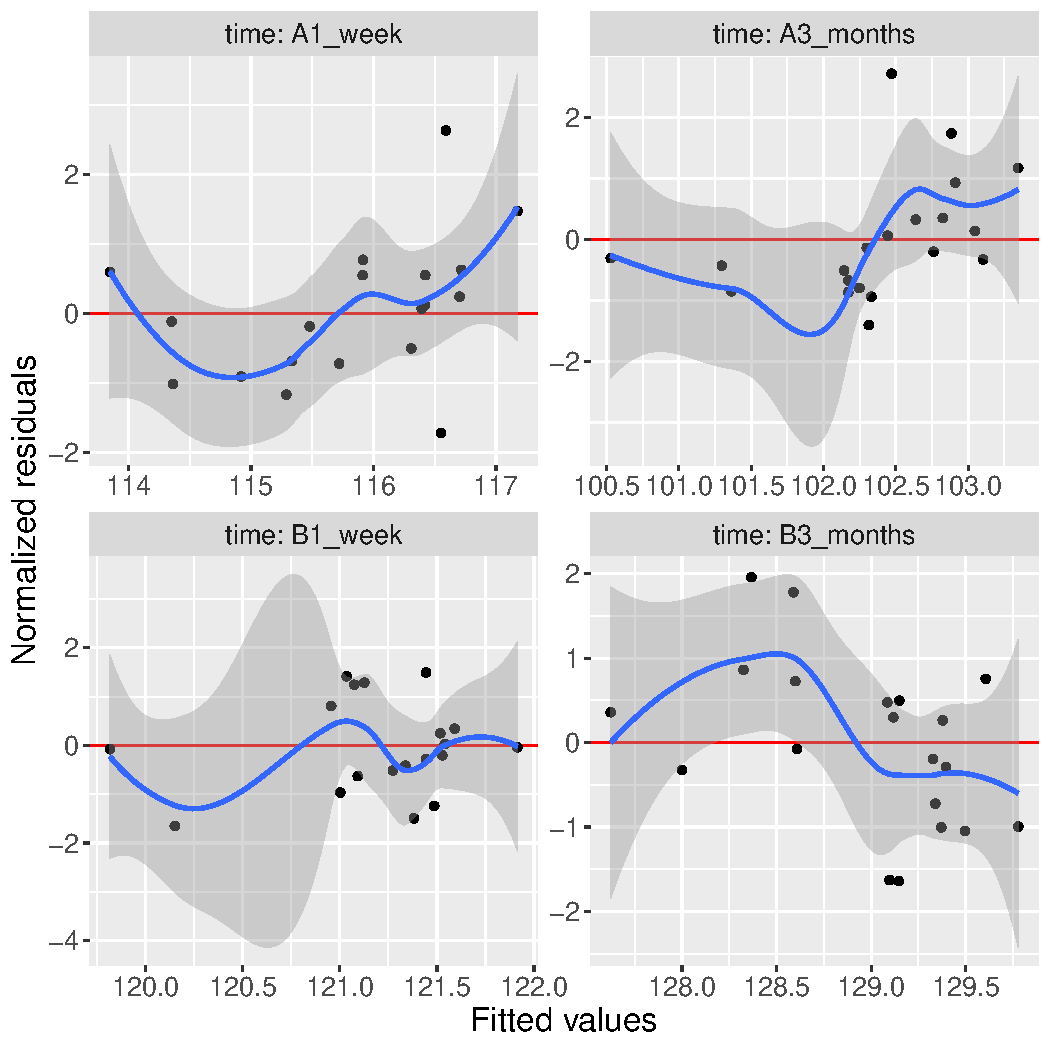
\includegraphics[width=0.4\textwidth]{./figures/diag-scatterplot.pdf}
\end{center}

\begin{itemize}
\item misspecification of the variance structure
\end{itemize}
\lstset{language=r,label= ,caption= ,captionpos=b,numbers=none}
\begin{lstlisting}
plot(eUN.lmm, type = "scatterplot2")
\end{lstlisting}

\begin{center}
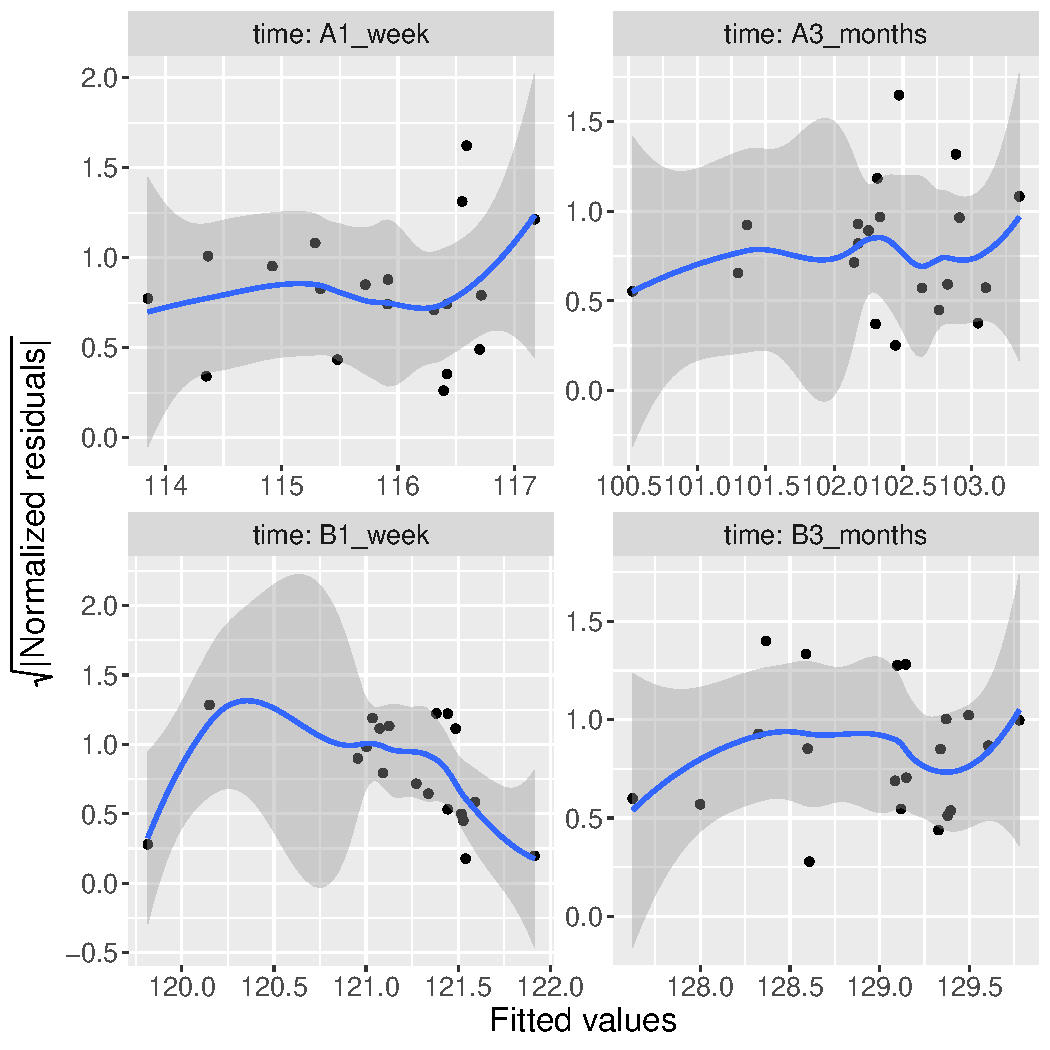
\includegraphics[width=0.4\textwidth]{./figures/diag-scatterplot2.pdf}
\end{center}

\clearpage

\begin{itemize}
\item misspecification of the correlation structure
\end{itemize}

\lstset{language=r,label= ,caption= ,captionpos=b,numbers=none}
\begin{lstlisting}
plot(eUN.lmm, type = "correlation", type.residual = "response")
plot(eUN.lmm, type = "correlation", type.residual = "normalized")
\end{lstlisting}

\begin{center}
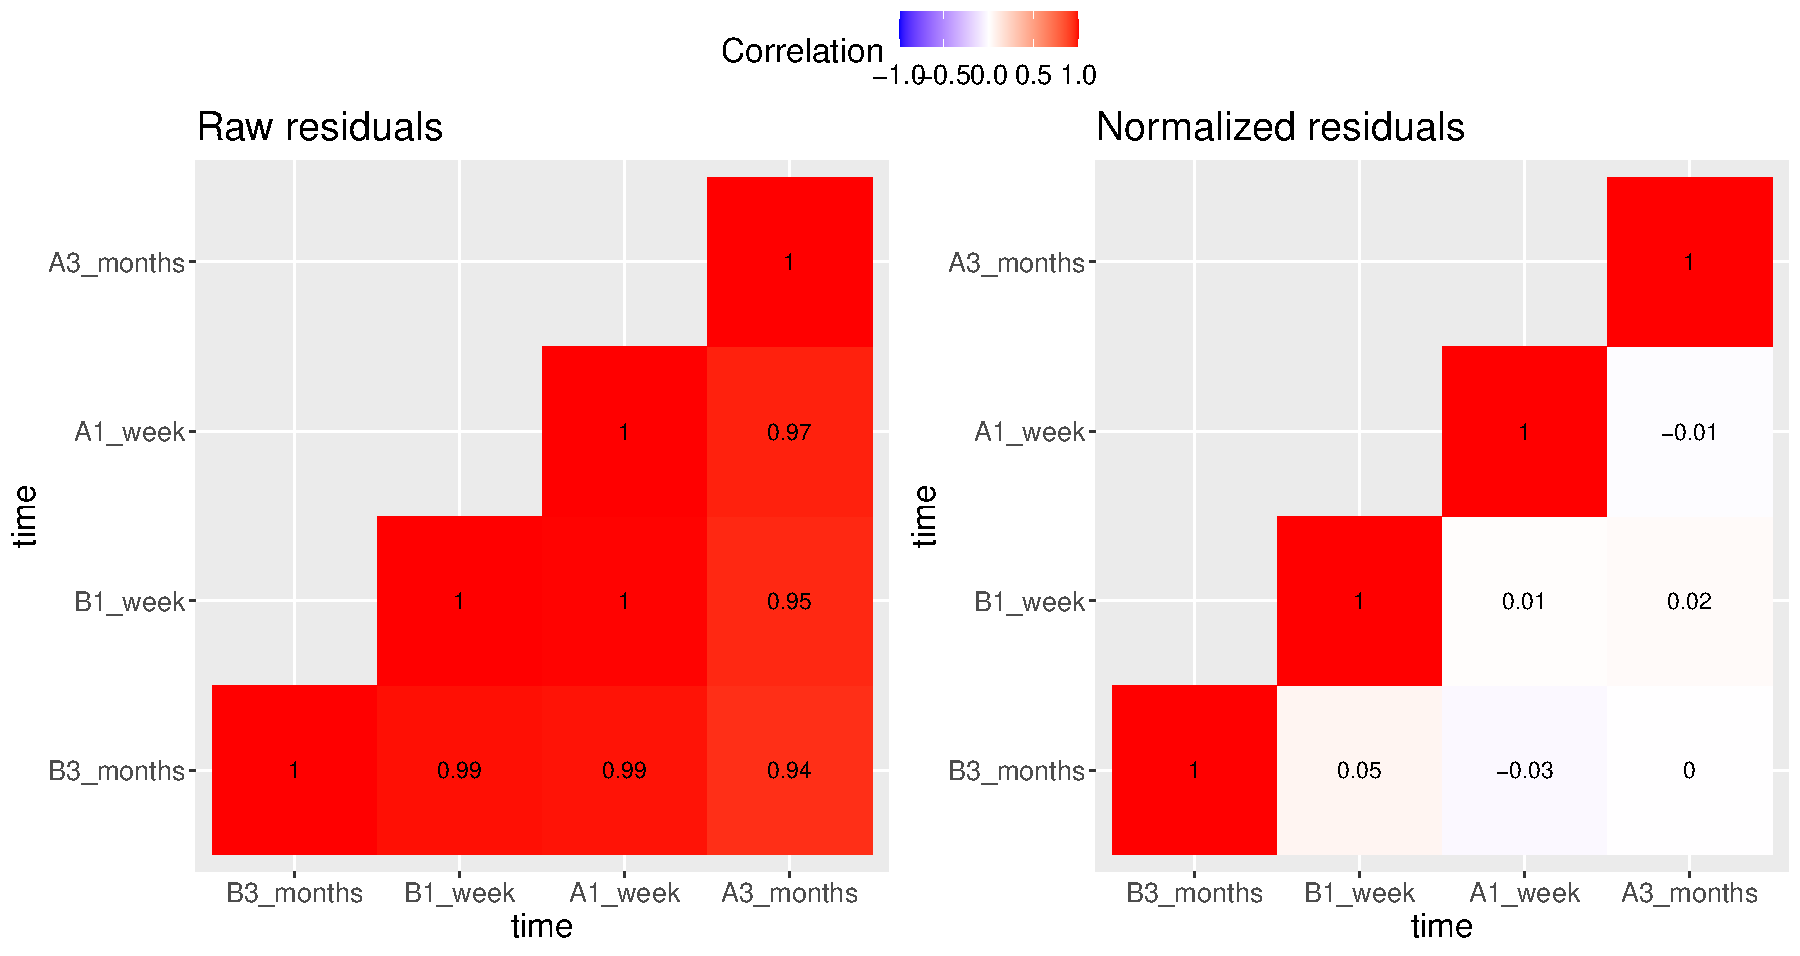
\includegraphics[width=0.6\textwidth]{./figures/diag-correlation.pdf}
\end{center}

\begin{itemize}
\item residual distribution vs. normal distribution \footnote{see \cite{oldford2016self} for guidance
about how to read quantile-quantile plots.}:
\end{itemize}
\lstset{language=r,label= ,caption= ,captionpos=b,numbers=none}
\begin{lstlisting}
plot(eUN.lmm, type = "qqplot", engine.qqplot = "qqtest")
## Note: the qqtest package to be installed to use the argument engine.plot = "qqtest" 
\end{lstlisting}

\begin{center}
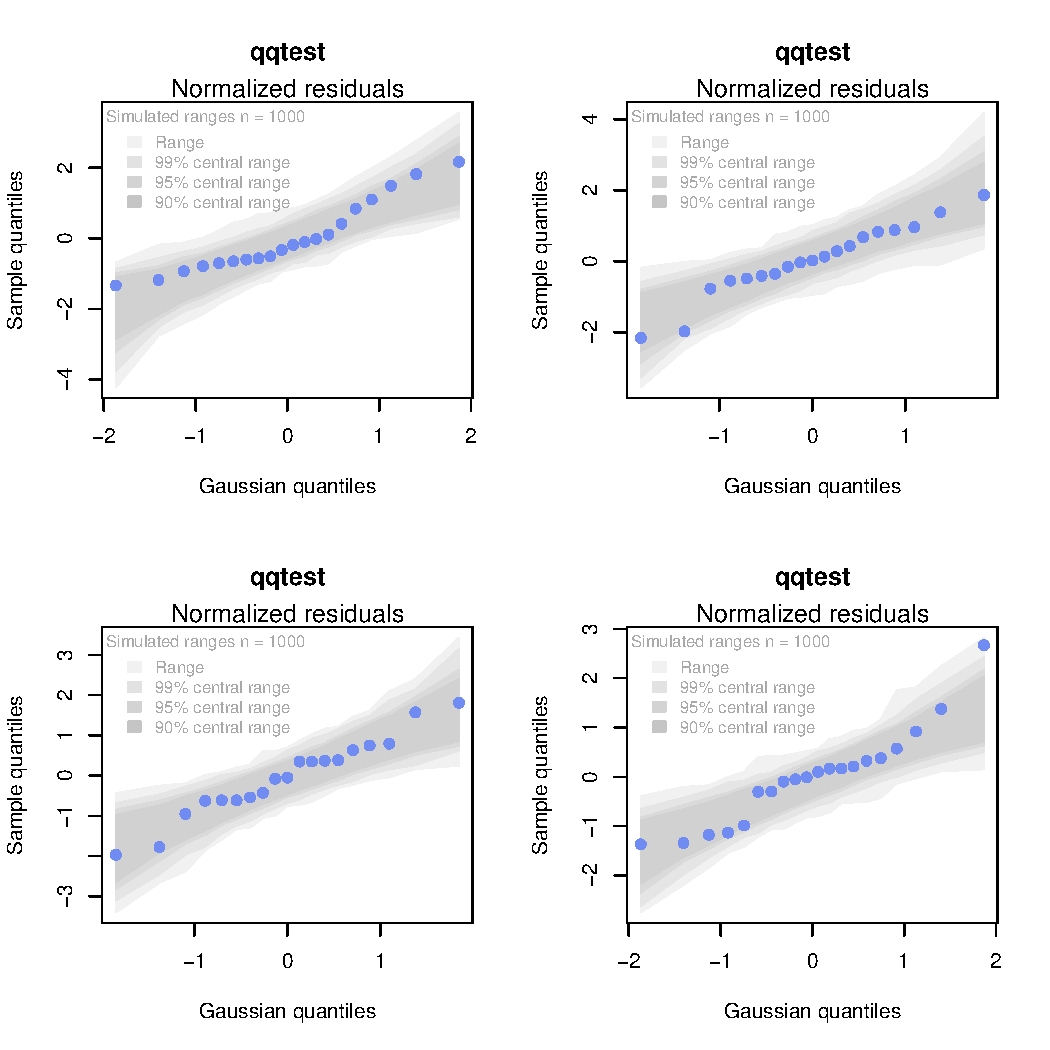
\includegraphics[width=0.5\textwidth]{./figures/diag-qqplot.pdf}
\end{center}

\clearpage

The method \texttt{residuals} returns the residulas in the wide format:
\lstset{language=r,label= ,caption= ,captionpos=b,numbers=none}
\begin{lstlisting}
eUN.diagW <- residuals(eUN.lmm, type = "normalized", format = "wide")
colnames(eUN.diagW) <- gsub("normalized.","",colnames(eUN.diagW))
head(eUN.diagW)
\end{lstlisting}

\begin{verbatim}
windows 
      2
  cluster      r.B3m      r.B1w       r.A1w      r.A3m
1       1 -0.2897365 -0.2027622 -1.16864038  0.3258573
2       2  0.8603117 -1.6492164  0.62578801  1.7370660
3       3  0.7273066 -0.4155171 -0.68266741 -0.8510316
4       4 -1.6403082 -0.5128368  0.06806206  1.1725813
5       5  0.4755409         NA -0.18736415 -0.8634200
6       6  1.7801675  1.2847703  2.63004812  0.3505542
\end{verbatim}


or in the long format:
\lstset{language=r,label= ,caption= ,captionpos=b,numbers=none}
\begin{lstlisting}
eUN.diagL <- residuals(eUN.lmm, type = "normalized", format = "long")
head(eUN.diagL)
\end{lstlisting}

\begin{verbatim}
[1] -0.2897365  0.8603117  0.7273066 -1.6403082  0.4755409  1.7801675
\end{verbatim}


Various type of residuals can be extract but the normalized one are
recommanded when doing model checking.

\subsection{Model fit}
\label{sec:org0a90a9a}

The fitted values can be displayed via the \texttt{plot} method or using the \texttt{emmeans} package:

\lstset{language=r,label= ,caption= ,captionpos=b,numbers=none}
\begin{lstlisting}
library(ggplot2) ## left panel
plot(eUN.lmm, type = "fit", color = "id", ci.alpha = NA, size.text = 20)
\end{lstlisting}

\lstset{language=r,label= ,caption= ,captionpos=b,numbers=none}
\begin{lstlisting}
library(emmeans) ## right panel
emmip(eUN.lmm, ~time) + theme(text = element_text(size=20))
\end{lstlisting}

\begin{minipage}{0.45\linewidth}
\begin{center}
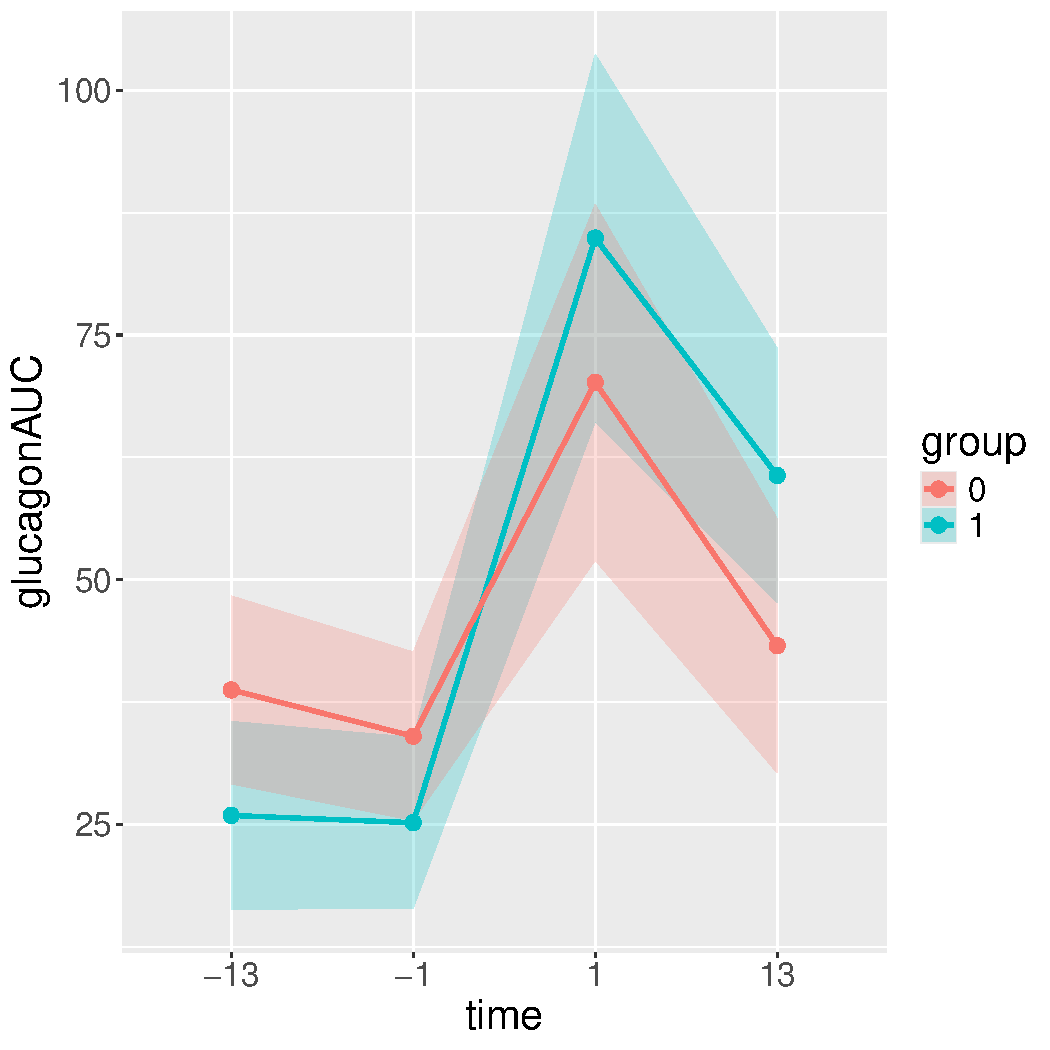
\includegraphics[width=\textwidth]{./figures/fit-autoplot.pdf}
\end{center}
\end{minipage}
\begin{minipage}{0.45\linewidth}
\begin{center}
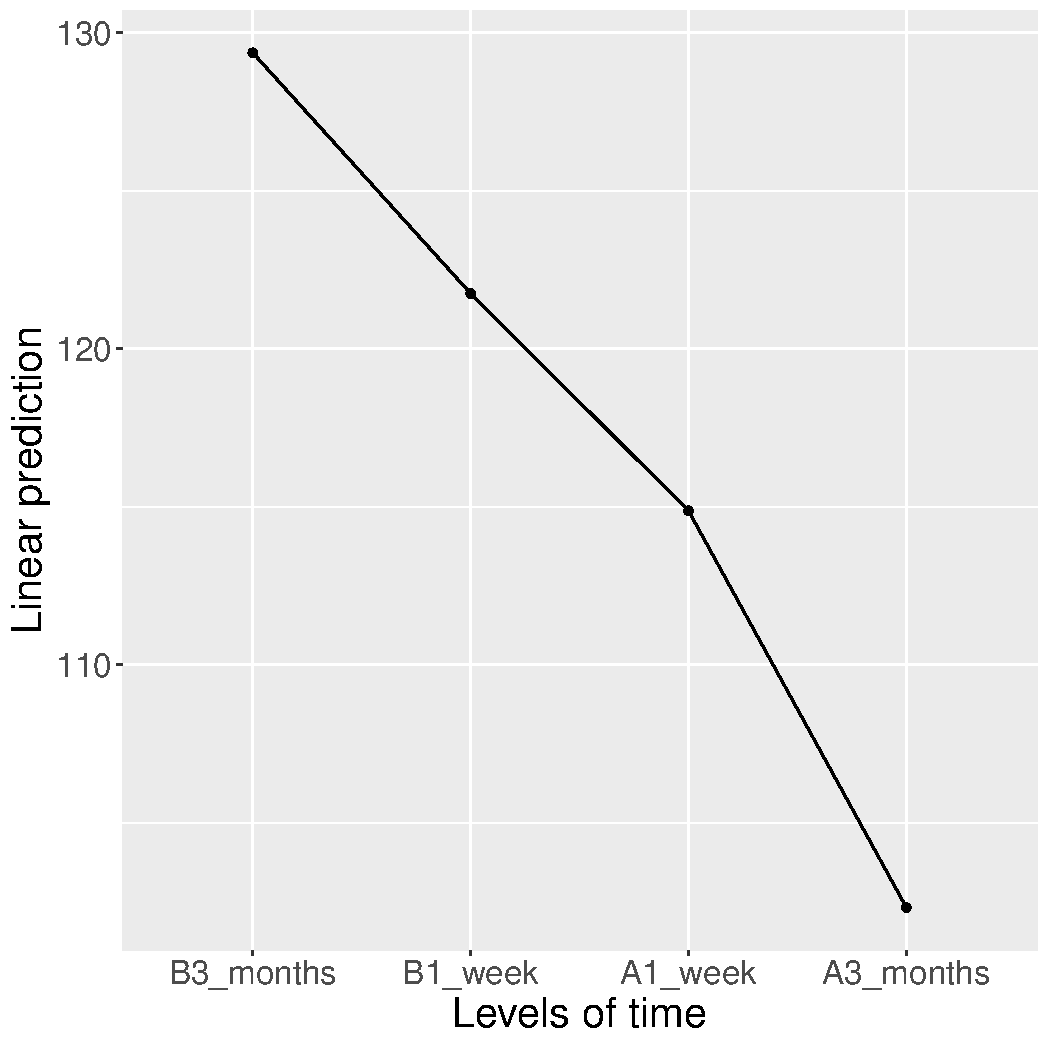
\includegraphics[width=\textwidth]{./figures/fit-emmip.pdf}
\end{center}
\end{minipage}

In the first case each possible curve is displayed while in the latter
the average curve (over glucagon values). With the \texttt{plot} method,
it is possible to display a curve specific to a glucagon value via the
argument \texttt{at}:
\lstset{language=r,label= ,caption= ,captionpos=b,numbers=none}
\begin{lstlisting}
plot(eUN.lmm, type = "fit", at = data.frame(glucagon = 10), color = "glucagon")
\end{lstlisting}

It is also possible to display the observed values along with the
fitted values by setting the argument \texttt{obs.alpha} to a strictly
positive value below or equal to 1. This argument controls the
transparency of the color used to display the observed values:
\lstset{language=r,label= ,caption= ,captionpos=b,numbers=none}
\begin{lstlisting}
  gg <- plot(eUN.lmm, type = "fit", obs.alpha = 0.2, ci = FALSE,plot = FALSE)$plot
  gg <- gg + facet_wrap(~id, labeller = label_both)
  gg <- gg + theme(axis.text.x=element_text(angle = 90, hjust = 0))
  gg
ggsave(gg + theme(text = element_text(size=20)), filename = "figures/fit-autoplot-indiv.pdf", width = 12)
\end{lstlisting}

\begin{center}
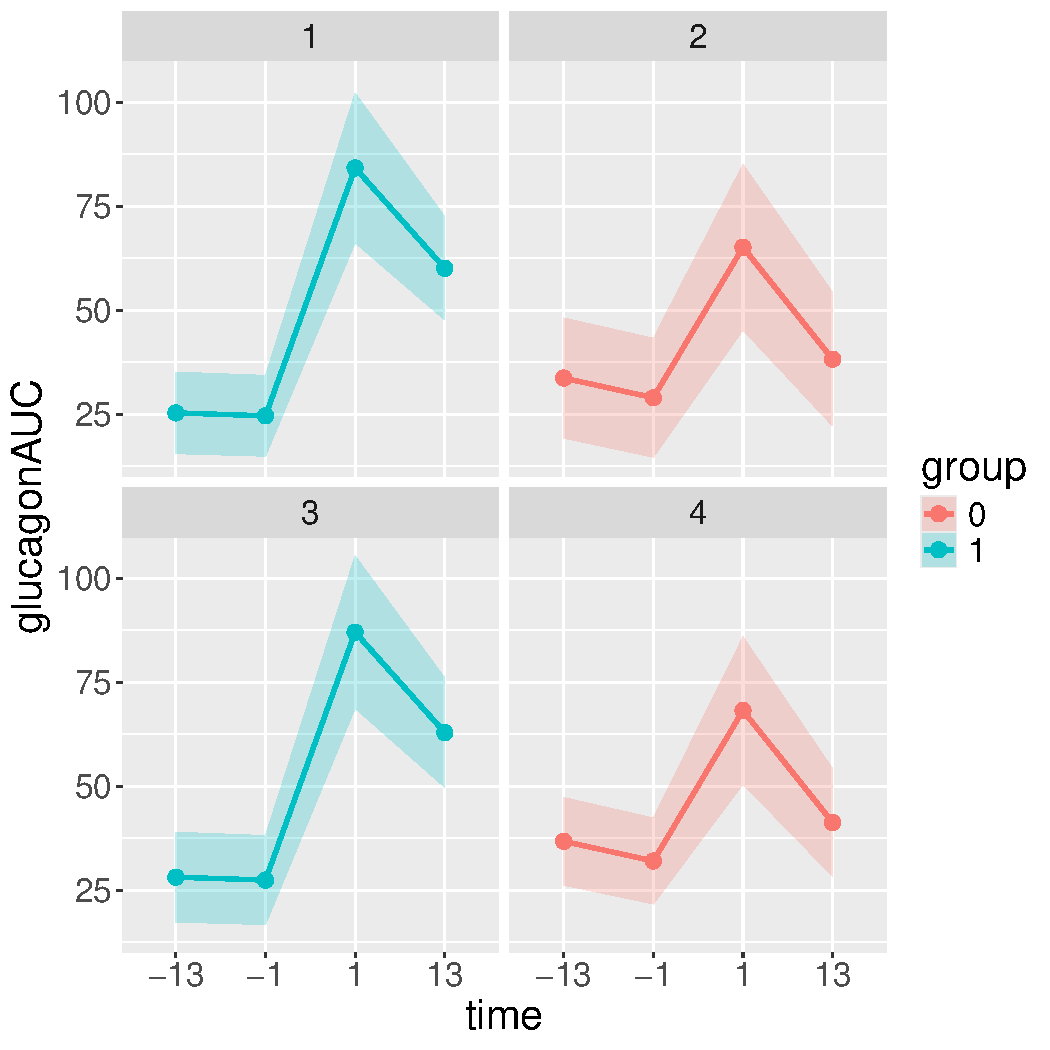
\includegraphics[width=\textwidth]{./figures/fit-autoplot-indiv.pdf}
\end{center}

\clearpage

Partial residuals can also be displayed via the \texttt{plot} method:
\lstset{language=r,label= ,caption= ,captionpos=b,numbers=none}
\begin{lstlisting}
gg1 <- plot(eUN.lmm, type = "partial", var = "glucagon", plot = FALSE)$plot
gg2 <- plot(eUN.lmm, type = "partial", var = c("(Intercept)","glucagon"), plot = FALSE)$plot
ggarrange(gg1,gg2)
\end{lstlisting}

\begin{center}
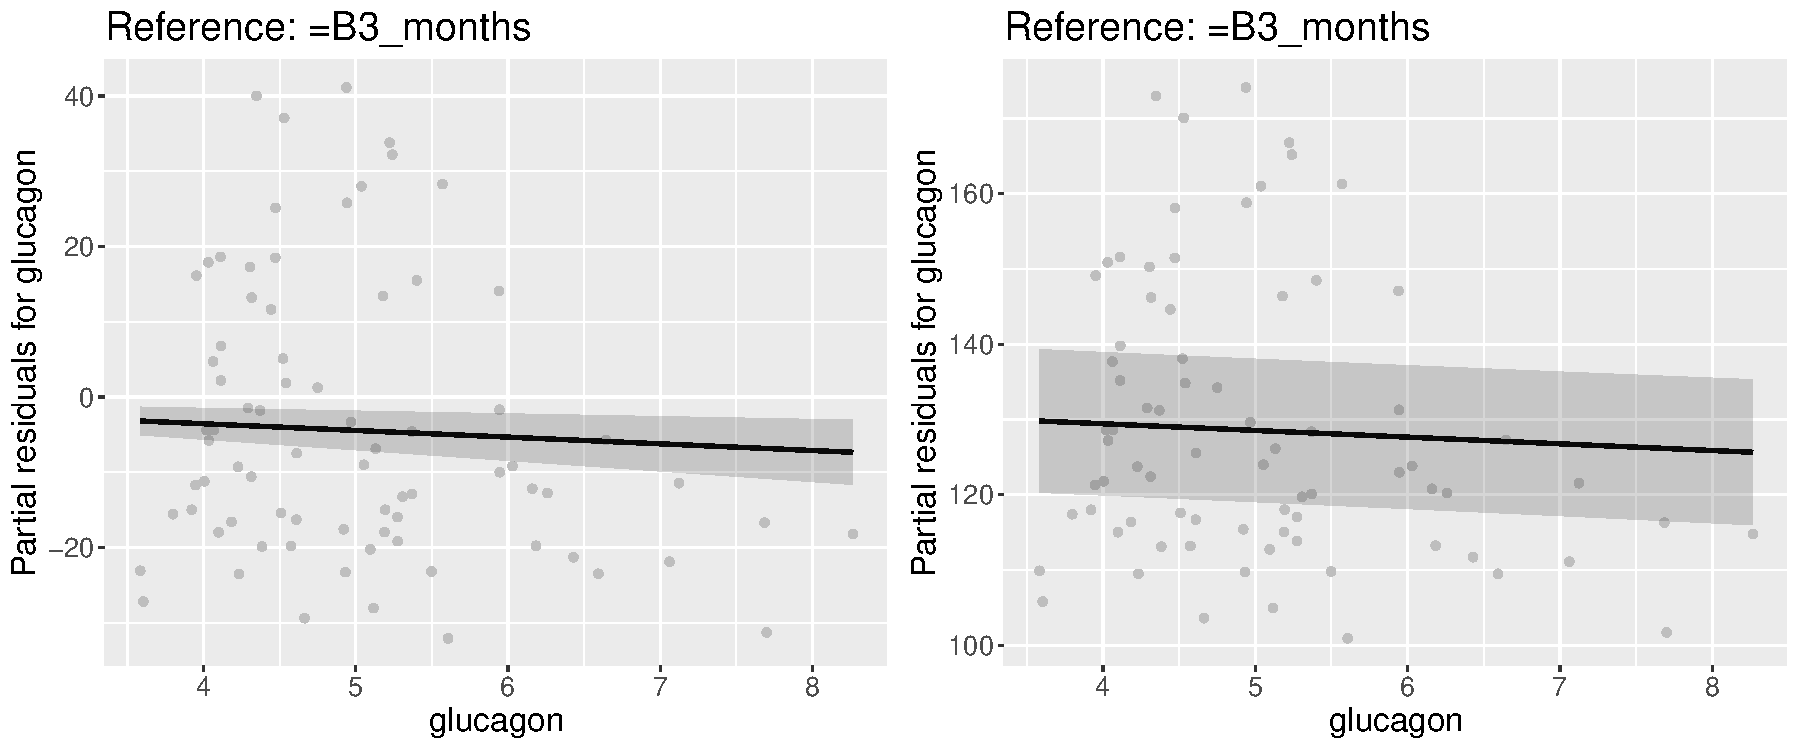
\includegraphics[width=\textwidth]{./figures/fit-pres.pdf}
\end{center}

Their value can be extracted via the \texttt{residuals} method, e.g.:
\lstset{language=r,label= ,caption= ,captionpos=b,numbers=none}
\begin{lstlisting}
df.pres <- residuals(eUN.lmm, type = "partial", var = "glucagon", keep.data = TRUE)
m.pres <- gastricbypassL$weight - model.matrix(~time,gastricbypassL) %*% coef(eUN.lmm)[1:4]
range(df.pres$r.partial - m.pres, na.rm = TRUE)
\end{lstlisting}

\begin{verbatim}
windows 
      2 
Advarselsbeskeder:
1: Removed 2 rows containing missing values (geom_point). 
2: Removed 2 row(s) containing missing values (geom_path). 
3: Removed 2 rows containing missing values (geom_point). 
4: Removed 2 row(s) containing missing values (geom_path).
[1] -1.421085e-14  1.421085e-14
\end{verbatim}


\clearpage

\subsection{Statistical inference (linear)}
\label{sec:orgeb7ecf8}

The \texttt{anova} method can be use to test one or several linear
combinations of the model coefficients using Wald tests. By default,
it will simultaneously test all parameters associated to a variable:
\lstset{language=r,label= ,caption= ,captionpos=b,numbers=none}
\begin{lstlisting}
anova(eUN.lmm)
\end{lstlisting}

\begin{verbatim}

	|| mean coefficients || 

 - Multivariate Wald test (global null hypothesis)
         F-statistic df.num df.denom    p.value    
time          86.743      3   19.005 2.8424e-11 ***
glucagon      13.518      1   13.708  0.0025716  **
---
 Signif. codes:  0 '***' 0.001 '**' 0.01 '*' 0.05 '.' 0.1 ' ' 1
\end{verbatim}


Note that here the p-values are not adjust for multiple comparisons
over variables. It is possible to specify a null hypothesis to be
test: e.g. is there a change in average weight just after taking the
treatment:
\lstset{language=r,label= ,caption= ,captionpos=b,numbers=none}
\begin{lstlisting}
anova(eUN.lmm, effects = c("timeA1w-timeB1w=0"))
\end{lstlisting}

\begin{verbatim}

	|| User-specified linear hypotheses || 

 - Multivariate Wald test (global null hypothesis)
 F-statistic df.num df.denom    p.value    
      43.141      1   17.875 3.7234e-06 ***
---
 Signif. codes:  0 '***' 0.001 '**' 0.01 '*' 0.05 '.' 0.1 ' ' 1
\end{verbatim}


One can also simulateneously tests several null hypotheses:
\lstset{language=r,label= ,caption= ,captionpos=b,numbers=none}
\begin{lstlisting}
e.anova <- anova(eUN.lmm, effects = c("timeA1w-timeB1w=0","timeA3m-timeB1w=0"))
summary(e.anova)
\end{lstlisting}

\begin{verbatim}

	|| User-specified linear hypotheses || 

 - Multivariate Wald test (global null hypothesis)
 F-statistic df.num df.denom    p.value    
      98.651      2    18.62 1.2338e-10 ***

 - Univariate Wald test (individual null hypotheses) 
                   estimate        se        df     lower   upper p.value    
timeA1w - timeB1w  -3.90572   0.59464  17.87453  -5.32146  -2.490   2e-05 ***
timeA3m - timeB1w -18.24016   1.32283  19.02810 -21.38959 -15.091  <1e-05 ***
---
Signif. codes:  0 '***' 0.001 '**' 0.01 '*' 0.05 '.' 0.1 ' ' 1
Standard errors: model-based
(CIs/p-values adjusted for multiple comparisons -- max-test adjustment)
Adjusted CIs/p-values computed using 1e+05 samples.
\end{verbatim}

or return all pairwise comparisons for a given factor using the \texttt{mcp}
function of the multcomp package:
\lstset{language=r,label= ,caption= ,captionpos=b,numbers=none}
\begin{lstlisting}
library(multcomp)
summary(anova(eUN.lmm, effects = mcp(time = "Tukey")))
\end{lstlisting}

\begin{verbatim}
Singular contrast matrix: contrasts "A1w - B1w" "A3m - B1w" "A3m - A1w" have been removed. 


	|| User-specified linear hypotheses || 

 - Multivariate Wald test (global null hypothesis)
 F-statistic df.num df.denom    p.value    
      86.743      3   19.005 2.8424e-11 ***

 - Univariate Wald test (individual null hypotheses) 
           estimate        se        df     lower    upper p.value    
B1w - B3m  -7.88223   0.71318  19.17147  -9.82458  -5.9399  <1e-05 ***
A1w - B3m -11.78795   1.01751  21.64404 -14.55916  -9.0168  <1e-05 ***
A3m - B3m -26.12239   1.65641  18.84049 -30.63363 -21.6112  <1e-05 ***
A1w - B1w  -3.90572   0.59464  17.87453  -5.52523  -2.2862   3e-05 ***
A3m - B1w -18.24016   1.32283  19.02810 -21.84289 -14.6374  <1e-05 ***
A3m - A1w -14.33444   1.05650  20.26658 -17.21182 -11.4571  <1e-05 ***
---
Signif. codes:  0 '***' 0.001 '**' 0.01 '*' 0.05 '.' 0.1 ' ' 1
Standard errors: model-based
(CIs/p-values adjusted for multiple comparisons -- max-test adjustment)
Adjusted CIs/p-values computed using 1e+05 samples.
\end{verbatim}


When testing transformed variance or correlation parameters,
parentheses (as in \texttt{log(k).B1w}) cause problem for recognizing
parameters:
\lstset{language=r,label= ,caption= ,captionpos=b,numbers=none}
\begin{lstlisting}
try(
  anova(eUN.lmm,
	effects = c("log(k).B1w=0","log(k).A1w=0","log(k).A3m=0"))
)
\end{lstlisting}

\begin{verbatim}
Error in .anova_Wald(object, effects = effects, robust = robust, rhs = rhs,  : 
  Possible mispecification of the argument 'effects' as running mulcomp::glht lead to the following error: 
Error in parse(text = ex[i]) : <text>:1:7: uventet symbol
1: log(k).B1w
          ^
\end{verbatim}


It is then advised to build a contrast matrix, e.g.:
\lstset{language=r,label= ,caption= ,captionpos=b,numbers=none}
\begin{lstlisting}
name.coef <- rownames(confint(eUN.lmm, effects = "all"))
name.varcoef <- grep("^k",name.coef, value = TRUE)
C <- matrix(0, nrow = 3, ncol = length(name.coef), dimnames = list(name.varcoef, name.coef))
diag(C[name.varcoef,name.varcoef]) <- 1
C
\end{lstlisting}

\begin{verbatim}
      (Intercept) timeB1w timeA1w timeA3m glucagon sigma k.B1w k.A1w k.A3m rho(B3m,B1w)
k.B1w           0       0       0       0        0     0     1     0     0            0
k.A1w           0       0       0       0        0     0     0     1     0            0
k.A3m           0       0       0       0        0     0     0     0     1            0
      rho(B3m,A1w) rho(B3m,A3m) rho(B1w,A1w) rho(B1w,A3m) rho(A1w,A3m)
k.B1w            0            0            0            0            0
k.A1w            0            0            0            0            0
k.A3m            0            0            0            0            0
\end{verbatim}


And then call the \texttt{anova} method specifying the null hypothesis via the
contrast matrix:
\lstset{language=r,label= ,caption= ,captionpos=b,numbers=none}
\begin{lstlisting}
anova(eUN.lmm, effects = C)
\end{lstlisting}

\begin{verbatim}

	|| User-specified linear hypotheses || 

 - Multivariate Wald test (global null hypothesis)
 F-statistic df.num df.denom   p.value   
      6.2032      3   17.995 0.0044171 **
---
 Signif. codes:  0 '***' 0.001 '**' 0.01 '*' 0.05 '.' 0.1 ' ' 1
\end{verbatim}


Note that using the approach of \cite{pipper2012versatile} it is also
possible to adjust for multiple testing across several \texttt{lmm}
objects. To do so, one first fit the mixed models, then use the
\texttt{anova} method to indicate which hypotheses are being tested, and
combine them using \texttt{rbind}. Here is an (artificial) example:
\lstset{language=r,label= ,caption= ,captionpos=b,numbers=none}
\begin{lstlisting}
Manova <- rbind(anova(eInd.lmm, effects = "glucagon = 0"),
		anova(eCS.lmm, effects = "glucagon = 0"),
		anova(eUN.lmm, effects = "glucagon = 0"),
		name = c("Ind","CS","UN"))
summary(Manova) 
\end{lstlisting}

\begin{verbatim}

	|| User-specified linear hypotheses || 

 - Multivariate Wald test (global null hypothesis)
 chi2-statistic df.num df.denom    p.value    
         8.8925      3      Inf 6.8788e-06 ***

 - Univariate Wald test (individual null hypotheses) 
               estimate        se        df     lower   upper p.value   
Ind: glucagon  -8.27006   2.57880  34.20071 -14.86149 -1.6786 0.01181 * 
CS: glucagon    0.82179   0.61997  53.80983  -0.76285  2.4064 0.47313   
UN: glucagon   -0.88831   0.24161  13.70759  -1.50586 -0.2708 0.00394 **
---
Signif. codes:  0 '***' 0.001 '**' 0.01 '*' 0.05 '.' 0.1 ' ' 1
Standard errors: model-based
(CIs/p-values adjusted for multiple comparisons -- max-test adjustment)
Adjusted CIs/p-values computed using 1e+05 samples.
\end{verbatim}

\clearpage

\subsection{Statistical inference (non-linear)}
\label{sec:orgec91b34}

The \texttt{estimate} function can be used to test one or several non-linear
combinations of model coefficients, using a first order delta method
to quantify uncertainty. The combination has to be specified via a
function (argument \texttt{f}). To illustrate its use consider an ANCOVA
analysis:
\[ Y_{i1} = \textcolor{\darkred}{\alpha} + \textcolor{\darkblue}{\beta} Y_{i,0} + \textcolor{\darkgreen}{\gamma} X_{i} + e_{i} \]

\lstset{language=r,label= ,caption= ,captionpos=b,numbers=none}
\begin{lstlisting}
gastricbypassW <- reshape(gastricbypassL[,c("id","time","weight","group")],
			  direction = "wide",
			  timevar = "time", idvar = c("id","group"))
e.ANCOVA <- lm(weight.A1w ~ weight.B1w + group, data = gastricbypassW)
summary(e.ANCOVA)$coef
\end{lstlisting}

\begin{verbatim}
              Estimate Std. Error    t value     Pr(>|t|)
(Intercept) -1.4823022 2.31781138 -0.6395267 5.310047e-01
weight.B1w   0.9654917 0.01803988 53.5198489 2.156258e-20
group        0.2521714 0.66499945  0.3792054 7.092302e-01
\end{verbatim}


We can replicate this analysis by first fitting a mixed model:
\[ Y_{ij} = \alpha_j + \gamma_j X_{i} + \varepsilon_{i,j} \text{ where } \varepsilon_i \sim \Gaus \left( \begin{bmatrix} 0 \\ 0 \end{bmatrix}, \begin{bmatrix} \sigma^2_1 & \rho \sigma_1 \sigma_2 \\ \rho \sigma_1 \sigma_2 & \sigma^2_2 \end{bmatrix} \right) \]
\lstset{language=r,label= ,caption= ,captionpos=b,numbers=none}
\begin{lstlisting}
e.lmmANCOVA <- lmm(weight ~ time+time:group, repetition = ~time|id,
		   data = gastricbypassL[gastricbypassL$visit %in% 2:3,])
\end{lstlisting}

and then perform a delta-method:
\lstset{language=r,label= ,caption= ,captionpos=b,numbers=none}
\begin{lstlisting}
lava::estimate(e.lmmANCOVA, f = function(p){
  c(Y1 = as.double(p["rho(B1w,A1w)"]*p["k.A1w"]),
    X1 = as.double(p["timeA1w:group"]-p["rho(B1w,A1w)"]*p["k.A1w"]*p["timeB1w:group"]))
})
\end{lstlisting}

\begin{verbatim}
    estimate         se       df      lower    upper   p.value
Y1 0.9654917 0.01753161 15.96769  0.9283203 1.002663 0.0000000
X1 0.2521714 0.64626331 15.00349 -1.1252784 1.629621 0.7018731
\end{verbatim}


Indeed:
\begin{align*}
\Esp[Y_{i2}|Y_{i1},X_{i}] &= \alpha_2 + \gamma_2 X_{i} + \rho \frac{\sigma_2}{\sigma_1}\left(Y_{i1} - \alpha_1 - \gamma_1 X_{i}\right) \\
                         &= \textcolor{\darkred}{\alpha_2 - \rho \frac{\sigma_2}{\sigma_1} \alpha_1}
                         + \textcolor{\darkblue}{\rho \frac{\sigma_2}{\sigma_1}Y_{i1}}
                         + \textcolor{\darkgreen}{\left(\gamma_2 - \rho \frac{\sigma_2}{\sigma_1} \gamma_1\right)  X_{i} }
\end{align*}

We obtain identical estimate but different standard-errors/degrees of
freedom compared to the univariate linear model approach. The later is
to be prefer as it does not rely on approximation. The former is
nevertheless useful as it can handle missing data in the outcome
variable.

\clearpage

\subsection{Baseline adjustment}
\label{sec:orge7a04db}

In clinical trial the group and intervention variable often do not
coincide, e.g., in presence of baseline measurement. In our running
example, the first two measurement are pre-treatment (i.e. treatment
should be \texttt{"none"}) while the last two measurements are post-treatment
(i.e. treatment should be \texttt{1} or \texttt{2}). The \texttt{baselineAdjustment}
function can be helpful to:
\begin{itemize}
\item define the treatment variable from the time and allocation variable, where baseline has its specific value
\end{itemize}
\lstset{language=r,label= ,caption= ,captionpos=b,numbers=none}
\begin{lstlisting}
gastricbypassL$treat <- baselineAdjustment(gastricbypassL, variable = "group",
					   repetition = ~time|id, constrain = c("B3m","B1w"),
					   new.level = "none")
table(treat = gastricbypassL$treat, time = gastricbypassL$time, group = gastricbypassL$group)
\end{lstlisting}

\begin{verbatim}
, , group = 0

      time
treat  B3m B1w A1w A3m
  none  10  10   0   0
  0      0   0  10  10
  1      0   0   0   0

, , group = 1

      time
treat  B3m B1w A1w A3m
  none  10  10   0   0
  0      0   0   0   0
  1      0   0  10  10
\end{verbatim}

\begin{itemize}
\item define the treatment variable from the time and allocation variable,
where baseline corresponds to the reference group
\end{itemize}
\lstset{language=r,label= ,caption= ,captionpos=b,numbers=none}
\begin{lstlisting}
gastricbypassL$treat2 <- baselineAdjustment(gastricbypassL, variable = "group",
					    repetition = ~time|id, constrain = c("B3m","B1w"))
table(treat = gastricbypassL$treat2, time = gastricbypassL$time, group = gastricbypassL$group)
\end{lstlisting}

\begin{verbatim}
, , group = 0

     time
treat B3m B1w A1w A3m
    1  10  10   0   0
    0   0   0  10  10

, , group = 1

     time
treat B3m B1w A1w A3m
    1  10  10  10  10
    0   0   0   0   0
\end{verbatim}

\begin{itemize}
\item define a time varying treatment variable from the time and allocation variable
\end{itemize}
\lstset{language=r,label= ,caption= ,captionpos=b,numbers=none}
\begin{lstlisting}
gastricbypassL$timeXtreat <- baselineAdjustment(gastricbypassL, variable = "group",
						repetition = ~time|id, constrain = c("B3m","B1w"),
						collapse.time = ".")

table(treat = gastricbypassL$timeXtreat, time = gastricbypassL$time, group = gastricbypassL$group)
\end{lstlisting}

\begin{verbatim}
, , group = 0

       time
treat   B3m B1w A1w A3m
  B3m    10   0   0   0
  B1w     0  10   0   0
  A1w.0   0   0  10   0
  A3m.0   0   0   0  10
  A1w.1   0   0   0   0
  A3m.1   0   0   0   0

, , group = 1

       time
treat   B3m B1w A1w A3m
  B3m    10   0   0   0
  B1w     0  10   0   0
  A1w.0   0   0   0   0
  A3m.0   0   0   0   0
  A1w.1   0   0  10   0
  A3m.1   0   0   0  10
\end{verbatim}

We would then typically like to model group differences only after
baseline (i.e. only at 1 week and 3 months after). This can be
performed using the time varying treatment variable, e.g.:
\lstset{language=r,label= ,caption= ,captionpos=b,numbers=none}
\begin{lstlisting}
eC.lmm <- lmm(weight ~ timeXtreat, data = gastricbypassL,
	      repetition = ~time|id, structure = "UN")
coef(eC.lmm) ## change from baseline
\end{lstlisting}

\begin{verbatim}
(Intercept)   timeXtreatB1w timeXtreatA1w.0 timeXtreatA3m.0 timeXtreatA1w.1 timeXtreatA3m.1 
  128.97000        -7.73000       -13.38978       -28.52130       -13.15022       -24.68870
\end{verbatim}


or
\lstset{language=r,label= ,caption= ,captionpos=b,numbers=none}
\begin{lstlisting}
eC2.lmm <- lmm(weight ~ 0 + timeXtreat, data = gastricbypassL,
	      repetition = ~time|id, structure = "UN")
coef(eC2.lmm) ## absolute value
\end{lstlisting}

\begin{verbatim}
timeXtreatB3m   timeXtreatB1w timeXtreatA1w.0 timeXtreatA3m.0 timeXtreatA1w.1 timeXtreatA3m.1 
     128.9700        121.2400        115.5802        100.4487        115.8198        104.2813
\end{verbatim}


The parametrization however does (directly) output treatment
effects. Instead one may be tempted to use a formula like
\texttt{treatment*time}. However this will lead to a non-indentifiable
model. Indeed we are only able to estimate a total of 6 means when
constraining the expected baseline value between the two groups to be
the same. Therefore can at most identify 6 effects. However the
design matrix for the interaction model:
\lstset{language=r,label= ,caption= ,captionpos=b,numbers=none}
\begin{lstlisting}
colnames(model.matrix(weight ~ treat*time, data = gastricbypassL))
\end{lstlisting}

\begin{verbatim}
 [1] "(Intercept)"    "treat0"         "treat1"         "timeB1w"        "timeA1w"       
 [6] "timeA3m"        "treat0:timeB1w" "treat1:timeB1w" "treat0:timeA1w" "treat1:timeA1w"
[11] "treat0:timeA3m" "treat1:timeA3m"
\end{verbatim}


contains 12 parameters (i.e. 6 too many). Fortunately, the \texttt{lmm}
contains an "experimental" feature to drop non-identifiable effects
from the model and will fit a simplified model:
\lstset{language=r,label= ,caption= ,captionpos=b,numbers=none}
\begin{lstlisting}
eC3.lmm <- lmm(weight ~ treat2*time, data = gastricbypassL,
	       repetition = ~time|id, structure = "UN")
\end{lstlisting}

\begin{verbatim}
Constant values in the design matrix in interactions "treat2:time"
 Coefficients "treat20" "treat20:timeB1w" have been removed.
\end{verbatim}


with the following coefficients:
\lstset{language=r,label= ,caption= ,captionpos=b,numbers=none}
\begin{lstlisting}
model.tables(eC3.lmm)
\end{lstlisting}

\begin{verbatim}
                estimate    se   df  lower  upper  p.value
(Intercept)       128.97 4.532 19.0 119.48 138.46 0.00e+00
timeB1w            -7.73 0.697 19.0  -9.19  -6.27 9.94e-10
timeA1w           -13.15 0.897 22.9 -15.01 -11.29 4.06e-13
timeA3m           -24.69 1.775 22.3 -28.37 -21.01 1.86e-12
treat20:timeA1w    -0.24 0.648 17.7  -1.60   1.12 7.16e-01
treat20:timeA3m    -3.83 2.107 17.6  -8.27   0.60 8.59e-02
\end{verbatim}


One can vizualize the baseline adjustment via the \texttt{autoplot} function:
\lstset{language=r,label= ,caption= ,captionpos=b,numbers=none}
\begin{lstlisting}
autoplot(eC3.lmm, color = "group", ci = FALSE, size.text = 20, obs.alpha = 0.1) 
\end{lstlisting}

\begin{center}
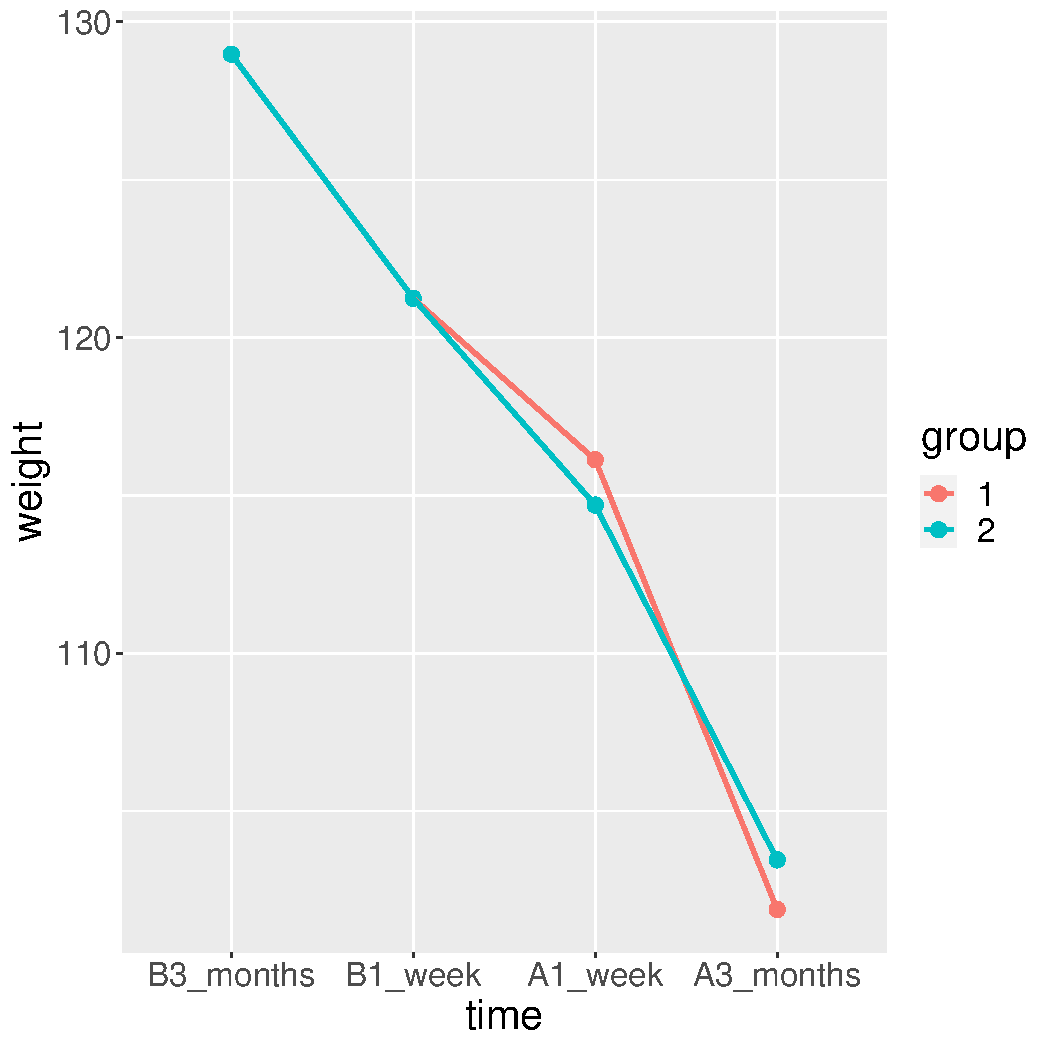
\includegraphics[width=0.4\textwidth]{./figures/gg-baseAdj.pdf}
\end{center}

\subsection{Marginal means}
\label{sec:org562bda6}

The \texttt{emmeans} package can be used to output marginal means. Consider
the following model:
\lstset{language=r,label= ,caption= ,captionpos=b,numbers=none}
\begin{lstlisting}
e.group <- lmm(weight ~ time*group, data = gastricbypassL,
	       repetition = ~time|id, structure = "UN")
\end{lstlisting}

We can for instance compute the average value over time \emph{assuming balanced groups}:
\lstset{language=r,label= ,caption= ,captionpos=b,numbers=none}
\begin{lstlisting}
emmeans(e.group, specs=~time)
\end{lstlisting}

\begin{verbatim}
NOTE: Results may be misleading due to involvement in interactions
 time emmean   SE df lower.CL upper.CL
 B3m     129 4.49 18    119.5      138
 B1w     121 4.20 18    112.4      130
 A1w     116 4.06 18    107.2      124
 A3m     102 3.88 18     94.2      111

Results are averaged over the levels of: group 
Confidence level used: 0.95
\end{verbatim}


This differs from the average value over time over the whole sample:
\lstset{language=r,label= ,caption= ,captionpos=b,numbers=none}
\begin{lstlisting}
df.pred <- cbind(gastricbypassL, predict(e.group, newdata = gastricbypassL))
summarize(formula = estimate~time, data = df.pred)
\end{lstlisting}

\begin{verbatim}
   outcome time observed missing    mean       sd    min  median    max
1 estimate  B3m       20       0 128.970 5.437685 123.67 128.970 134.27
2 estimate  B1w       20       0 121.240 4.873397 116.49 121.240 125.99
3 estimate  A1w       20       0 115.700 4.575863 111.24 115.700 120.16
4 estimate  A3m       20       0 102.365 2.354620 100.07 102.365 104.66
\end{verbatim}


as the groups are not balanced:
\lstset{language=r,label= ,caption= ,captionpos=b,numbers=none}
\begin{lstlisting}
table(group = gastricbypassL$group, time = gastricbypassL$time)
\end{lstlisting}

\begin{verbatim}
     time
group B3m B1w A1w A3m
    0  10  10  10  10
    1  10  10  10  10
\end{verbatim}


The "emmeans" approach gives equal "weight" to the expected value of
both group 2:
\lstset{language=r,label= ,caption= ,captionpos=b,numbers=none}
\begin{lstlisting}
mu.group1 <-  as.double(coef(e.group)["(Intercept)"])
mu.group2 <-  as.double(coef(e.group)["(Intercept)"] + coef(e.group)["group"])
p.group1 <- 14/20          ; p.group2 <- 6/20
c(emmeans = (mu.group1+mu.group2)/2, predict = mu.group1 * p.group1 + mu.group2 * p.group2)
\end{lstlisting}

\begin{verbatim}
emmeans predict 
 128.97  131.09
\end{verbatim}


Which one is relevant depends on the application. The \texttt{emmeans}
function can also be used to display expected value in each group over
time:
\lstset{language=r,label= ,caption= ,captionpos=b,numbers=none}
\begin{lstlisting}
emmeans.group <- emmeans(e.group, specs = ~group|time)
emmeans.group
\end{lstlisting}

\begin{verbatim}
time = B3m:
 group emmean   SE df lower.CL upper.CL
     0    134 6.34 18    120.9      148
     1    124 6.34 18    110.3      137

time = B1w:
 group emmean   SE df lower.CL upper.CL
     0    126 5.94 18    113.5      138
     1    116 5.94 18    104.0      129

time = A1w:
 group emmean   SE df lower.CL upper.CL
     0    120 5.75 18    108.1      132
     1    111 5.75 18     99.2      123

time = A3m:
 group emmean   SE df lower.CL upper.CL
     0    105 5.49 18     93.1      116
     1    100 5.49 18     88.5      112

Confidence level used: 0.95
\end{verbatim}

Using the \texttt{pair} function displays the differences:
\lstset{language=r,label= ,caption= ,captionpos=b,numbers=none}
\begin{lstlisting}
epairs.group <- pairs(emmeans.group, reverse = TRUE)
epairs.group
\end{lstlisting}

\begin{verbatim}
time = B3m:
 contrast estimate   SE df t.ratio p.value
 1 - 0      -10.60 8.97 18  -1.181  0.2528

time = B1w:
 contrast estimate   SE df t.ratio p.value
 1 - 0       -9.50 8.40 18  -1.132  0.2726

time = A1w:
 contrast estimate   SE df t.ratio p.value
 1 - 0       -8.92 8.13 18  -1.097  0.2870

time = A3m:
 contrast estimate   SE df t.ratio p.value
 1 - 0       -4.59 7.76 18  -0.591  0.5616
\end{verbatim}

One can adjust for multiple comparison via the \texttt{adjust} argument and
display confidence intervals setting the argument \texttt{infer} to \texttt{TRUE}:
\lstset{language=r,label= ,caption= ,captionpos=b,numbers=none}
\begin{lstlisting}
summary(epairs.group, by = NULL, adjust = "mvt", infer = TRUE)
\end{lstlisting}

\begin{verbatim}
 contrast time estimate   SE df lower.CL upper.CL t.ratio p.value
 1 - 0    B3m    -10.60 8.97 18    -30.9     9.69  -1.181  0.3158
 1 - 0    B1w     -9.50 8.40 18    -28.5     9.49  -1.132  0.3390
 1 - 0    A1w     -8.92 8.13 18    -27.3     9.47  -1.097  0.3561
 1 - 0    A3m     -4.59 7.76 18    -22.1    12.96  -0.591  0.6640

Confidence level used: 0.95 
Conf-level adjustment: mvt method for 4 estimates 
P value adjustment: mvt method for 4 tests
\end{verbatim}


This should also work when doing baseline adjustment (because of
baseline adjustment no difference is expected at the first two
timepoints):
\lstset{language=r,label= ,caption= ,captionpos=b,numbers=none}
\begin{lstlisting}
summary(pairs(emmeans(eC3.lmm , specs = ~treat2|time), reverse = TRUE), by = NULL)
\end{lstlisting}

\begin{verbatim}
Note: adjust = "tukey" was changed to "sidak"
because "tukey" is only appropriate for one set of pairwise comparisons
 contrast time estimate    SE   df t.ratio p.value
 0 - 1    B3m      0.00 0.000  NaN     NaN     NaN
 0 - 1    B1w      0.00 0.000  NaN     NaN     NaN
 0 - 1    A1w     -0.24 0.648 17.7  -0.369  0.9935
 0 - 1    A3m     -3.83 2.107 17.6  -1.819  0.3019

P value adjustment: sidak method for 4 tests
\end{verbatim}

\subsection{Predictions}
\label{sec:org9c3e8fb}

Two types of predictions can be performed with the \texttt{predict} method:
\begin{itemize}
\item \textbf{static predictions} that are only conditional on the covariates:
\end{itemize}
\lstset{language=r,label= ,caption= ,captionpos=b,numbers=none}
\begin{lstlisting}
news <- gastricbypassL[gastricbypassL$id==1,]
news$glucagon <- 0
predict(eUN.lmm, newdata = news)
\end{lstlisting}

\begin{verbatim}
  estimate       se       df     lower    upper
1 132.9801 4.664247 19.75815 123.24305 142.7172
2 125.0979 4.388294 19.91418 115.94155 134.2543
3 121.1922 4.214230 20.55331 112.41660 129.9678
4 106.8577 3.942058 20.95499  98.65871 115.0568
\end{verbatim}


\clearpage

which can be computing by creating a design matrix:
\lstset{language=r,label= ,caption= ,captionpos=b,numbers=none}
\begin{lstlisting}
X.12 <- model.matrix(formula(eUN.lmm), news)
X.12
\end{lstlisting}

\begin{verbatim}
   (Intercept) timeB1w timeA1w timeA3m glucagon
1            1       0       0       0        0
21           1       1       0       0        0
41           1       0       1       0        0
61           1       0       0       1        0
attr(,"assign")
[1] 0 1 1 1 2
attr(,"contrasts")
attr(,"contrasts")$time
[1] "contr.treatment"
\end{verbatim}

and then multiplying it with the regression coefficients:
\lstset{language=r,label= ,caption= ,captionpos=b,numbers=none}
\begin{lstlisting}
X.12 %*% coef(eUN.lmm)
\end{lstlisting}

\begin{verbatim}
       [,1]
1  132.9801
21 125.0979
41 121.1922
61 106.8577
\end{verbatim}


\begin{itemize}
\item \textbf{dynamic predictions} that are conditional on the covariates and the
outcome measured at other timepoints. Consider two subjects for who
we would like to predict the weight 1 week before the intervention
based on the weight 3 months before the intervention:
\end{itemize}

\lstset{language=r,label= ,caption= ,captionpos=b,numbers=none,otherkeywords={}, deletekeywords={}}
\begin{lstlisting}
newd <- rbind(
  data.frame(id = 1, time = "B3m", weight = coef(eUN.lmm)["(Intercept)"], glucagon = 0),
  data.frame(id = 1, time = "B1w", weight = NA, glucagon = 0),
  data.frame(id = 2, time = "B3m", weight = 100, glucagon = 0),
  data.frame(id = 2, time = "B1w", weight = NA, glucagon = 0)
)
predict(eUN.lmm, newdata = newd, type = "dynamic", keep.newdata = TRUE)
\end{lstlisting}

\begin{verbatim}
  id time   weight glucagon  estimate        se  df     lower    upper
1  1  B3m 132.9801        0        NA        NA  NA        NA       NA
2  1  B1w       NA        0 125.09790 0.6362754 Inf 123.85083 126.3450
3  2  B3m 100.0000        0        NA        NA  NA        NA       NA
4  2  B1w       NA        0  94.47017 7.2279385 Inf  80.30367 108.6367
\end{verbatim}


The first subjects has the average weight while the second has a much
  lower weight. The predicted weight for the first subject is then the
  average weight one week before while it is lower for the second
  subject due to the positive correlation over time. The predicted
  value is computed using the formula of the conditional mean for a
  Gaussian vector:
\lstset{language=r,label= ,caption= ,captionpos=b,numbers=none}
\begin{lstlisting}
mu1 <- coef(eUN.lmm)[1]
mu2 <- sum(coef(eUN.lmm)[1:2])
Omega_11 <- sigma(eUN.lmm)["B3m","B3m"]
Omega_21 <- sigma(eUN.lmm)["B1w","B3m"]
as.double(mu2 + Omega_21 * (100 - mu1) / Omega_11)
\end{lstlisting}

\begin{verbatim}
[1] 94.47017
\end{verbatim}



\clearpage

\subsection{Missing values and imputation}
\label{sec:orgf60bb04}


We now consider the glucagon level as an outcome. The \texttt{summarize}
function can be used to describe the amount of missing data at each
repetition:
\lstset{language=r,label= ,caption= ,captionpos=b,numbers=none}
\begin{lstlisting}
sss <- summarize(glucagon ~ time, data = gastricbypassL, na.rm = TRUE)
cbind(sss[,1:4], pc = paste0(100 * sss$missing / (sss$missing + sss$observed), "%"))
\end{lstlisting}

\begin{verbatim}
   outcome time observed missing pc
1 glucagon  B3m       20       0 0%
2 glucagon  B1w       19       1 5%
3 glucagon  A1w       19       1 5%
4 glucagon  A3m       20       0 0%
\end{verbatim}


Further description of the missing data patterns rely on function
outside the LMMstar package, e.g. appropriate call to \texttt{tapply} and
\texttt{table}:
\lstset{language=r,label= ,caption= ,captionpos=b,numbers=none}
\begin{lstlisting}
vec.pattern <- tapply(as.numeric(is.na(gastricbypassL$glucagon)),
		      INDEX = gastricbypassL$id,
		      FUN = paste, collapse=".")
table(vec.pattern)
\end{lstlisting}

\begin{verbatim}
vec.pattern
0.0.0.0 0.0.1.0 0.1.0.0 
     18       1       1
\end{verbatim}


Linear mixed model can handle missing value in the outcome variable,
assuming that missigness is random conditional on the covariate and
observed outcome values. The \texttt{lmm} function can be used "as usual":
\lstset{language=r,label= ,caption= ,captionpos=b,numbers=none}
\begin{lstlisting}
eUN.lmmNA <- lmm(glucagon ~ time,
		 repetition = ~time|id, structure = "UN",
		 data = gastricbypassL)
summary(eUN.lmmNA, hide.fit = TRUE,
	hide.cor = TRUE, hide.sd = TRUE, hide.mean = TRUE)
\end{lstlisting}

\begin{verbatim}
           Linear Mixed Model 
 
Dataset: gastricbypassL 

  - 20 clusters 
  - 78 observations were analyzed, 2 were excluded because of missing values 
  - between 3 and 4 observations per cluster 

Summary of the outcome and covariates: 

    $ glucagon: num  4.03 5.24 4.93 4.32 4.38 ...
    $ time    : Factor w/ 4 levels "B3m","B1w","A1w",..: 1 1 1 1 1 1 1 1 1 1 ...
    reference level: time=B3m
\end{verbatim}

The visible difference in the summary is when describing the dataset:
we can see that some repetitions (here 2) have been ignored as the
outcome was missing. So for some clusters only 3 values were analyzed
instead of 4. It is possible to extract the most likely value for
these missing observation using the \texttt{fitted} function with argument
\texttt{impute=TRUE}:
\lstset{language=r,label= ,caption= ,captionpos=b,numbers=none}
\begin{lstlisting}
fitted(eUN.lmmNA, impute = TRUE)
\end{lstlisting}

\begin{verbatim}
[1] 4.256984 6.497856
\end{verbatim}


When using the argument \texttt{keep.newdata=TRUE}, the missing outcome value
has been replaced by its most likely value (which is the same as the
dynamic prediction, describedy previously):
\lstset{language=r,label= ,caption= ,captionpos=b,numbers=none}
\begin{lstlisting}
eData <- fitted(eUN.lmmNA, impute = TRUE, keep.newdata = TRUE)
eData$treat <- eData$treat2 <- eData$timeXtreat <- NULL
eData[eData$id %in% eData[eData$imputed,"id"],]
\end{lstlisting}

\begin{verbatim}
   id visit time weight glucagonAUC baseline glucagon group imputed
5   5     1  B3m  113.1      7090.5     TRUE 4.383738     1   FALSE
15 15     1  B3m  115.0      5410.5     TRUE 4.098741     1   FALSE
25  5     2  B1w  105.6          NA     TRUE 4.256984     1    TRUE
35 15     2  B1w  109.7      7833.0     TRUE 4.509697     1   FALSE
45  5     3  A1w   99.9     19155.0    FALSE 6.430376     1   FALSE
55 15     3  A1w  103.5          NA    FALSE 6.497856     1    TRUE
65  5     4  A3m   87.7     12345.0    FALSE 5.275118     1   FALSE
75 15     4  A3m   94.1     18148.5    FALSE 6.259632     1   FALSE
\end{verbatim}


Visually:
\lstset{language=r,label= ,caption= ,captionpos=b,numbers=none}
\begin{lstlisting}
ggplot(eData, aes(x=time,y=glucagon, group=id)) + geom_line() + geom_point(aes(color=imputed))
\end{lstlisting}

\begin{center}
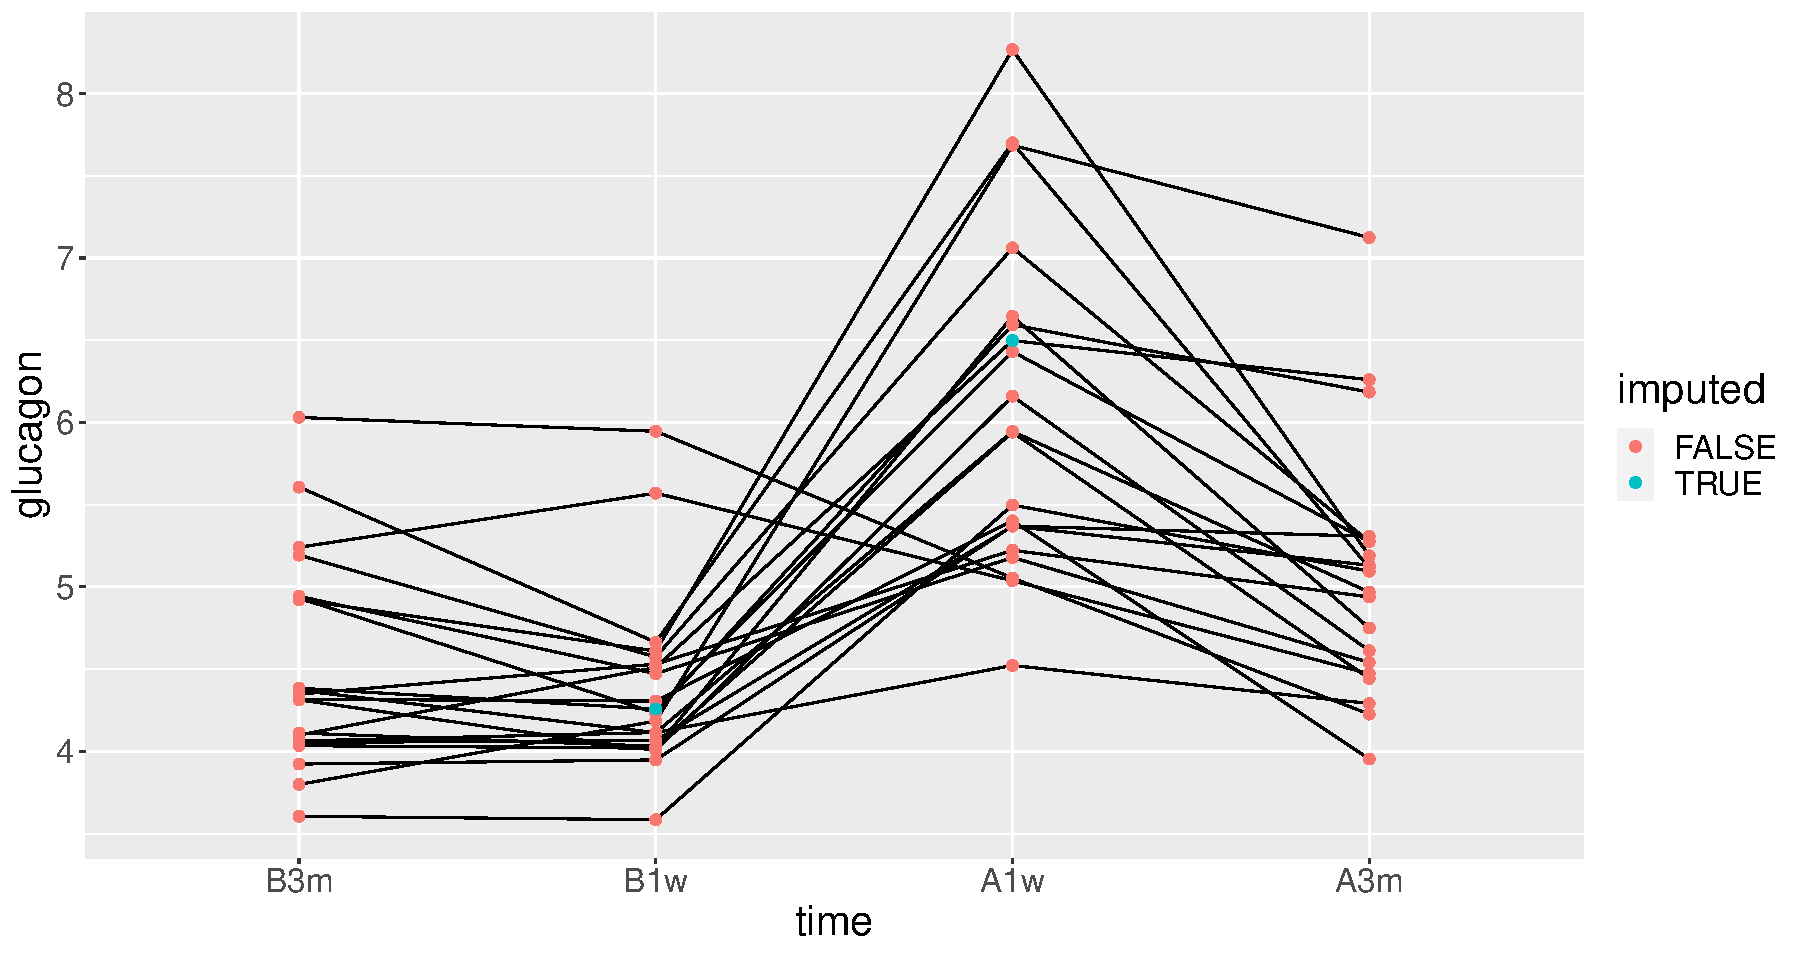
\includegraphics[trim={0 0 0 0},width=1\textwidth]{./figures/imputation.pdf}
\end{center}

It is possible to sample from the estimated distribution of the
missing value instead of using the most likely value, e.g. accounting
for residual variance and uncertainty related to parameter estimation:
\lstset{language=r,label= ,caption= ,captionpos=b,numbers=none}
\begin{lstlisting}
set.seed(10)
fitted(eUN.lmmNA, impute = TRUE, se = "total")
fitted(eUN.lmmNA, impute = TRUE, se = "total")
fitted(eUN.lmmNA, impute = TRUE, se = "total")
\end{lstlisting}

\begin{verbatim}
[1] 4.262434 6.305287
[1] 3.858267 5.871642
[1] 4.342624 6.905246
\end{verbatim}


\clearpage

\section{User-specific covariance patterns}
\label{sec:org50d3efe}

From version 0.6.0 and above it is possible customize the covariance
pattern under the following model for the residuals:
\[\Omega = \trans{\boldsymbol{\sigma}} R \boldsymbol{\sigma}\]
where:
\begin{itemize}
\item \(\boldsymbol{\sigma}=f(\boldsymbol{\theta}_{\sigma},Z_{\sigma})\)
is a vector of residual standard errors depending on a vector of
parameters \(\boldsymbol{\theta}_{\sigma}\) and possible covariates
via the design matrix \(Z_{\sigma}\).
\item \(R=g(\boldsymbol{\theta}_{R},Z_R)\) is a matrix of residual
correlations depending on a vector of parameters
\(\boldsymbol{\theta}_{R}\) and possible covariates via the design
matrix \(Z_R\).
\end{itemize}

\bigskip

To be more concrete, consider the following correlation matrix
\lstset{language=r,label= ,caption= ,captionpos=b,numbers=none}
\begin{lstlisting}
rho.2block <- function(p,time,...){
  n.time <- length(time)
  rho <- matrix(1, nrow = n.time, ncol = n.time)
  rho[1,2] <- rho[2,1] <- rho[4,5] <- rho[5,4] <- p["rho1"]
  rho[1,3] <- rho[3,1] <- rho[4,6] <- rho[6,4] <- p["rho2"]
  rho[2,3] <- rho[3,2] <- rho[5,6] <- rho[6,5] <- p["rho3"]
  rho[4:6,1:3] <- rho[1:3,4:6] <- p["rho4"]
  return(rho)
}
Rho <- rho.2block(p = c(rho1=0.25,rho2=0.5,rho3=0.4,rho4=0.1),
		  time = 1:6)
Rho
\end{lstlisting}

\begin{verbatim}
     [,1] [,2] [,3] [,4] [,5] [,6]
[1,] 1.00 0.25  0.5 0.10 0.10  0.1
[2,] 0.25 1.00  0.4 0.10 0.10  0.1
[3,] 0.50 0.40  1.0 0.10 0.10  0.1
[4,] 0.10 0.10  0.1 1.00 0.25  0.5
[5,] 0.10 0.10  0.1 0.25 1.00  0.4
[6,] 0.10 0.10  0.1 0.50 0.40  1.0
\end{verbatim}


and the corresponding dataset:
\lstset{language=r,label= ,caption= ,captionpos=b,numbers=none}
\begin{lstlisting}
set.seed(11)
n <- 1000
Y <- rmvnorm(n, mean = rep(0,6), sigma = Rho)
dfL <- reshape2::melt(cbind(id = 1:n, as.data.frame(Y)), id.vars = "id")
dfL$time  <- dfL$variable
dfL <- dfL[order(dfL$id),]
dfL[1:8,]
\end{lstlisting}

\begin{verbatim}
     id variable      value time
1     1       V1 -0.9842079   V1
1001  1       V2 -0.3681245   V2
2001  1       V3 -1.6174652   V3
3001  1       V4 -1.4994103   V4
4001  1       V5  0.7493107   V5
5001  1       V6 -1.0719657   V6
2     2       V1  1.2402726   V1
1002  2       V2  0.6494215   V2
\end{verbatim}


To fit the corresponding mixed model, we call \texttt{lmm} using a
(non-standard) correlation structure via the \texttt{CUSTOM} structure:
\lstset{language=r,label= ,caption= ,captionpos=b,numbers=none}
\begin{lstlisting}
e.lmmCUSTOM <- lmm(value~time,
		   repetition=~time|id,
		   structure=CUSTOM(~variable,
				    FCT.sigma = function(p,time,X){rep(p,length(time))}, ## function f
				    init.sigma = c("sigma"=1),
				    FCT.rho = rho.2block, ## function g
				    init.rho = c("rho1"=0.25,"rho2"=0.25,"rho3"=0.25,"rho4"=0.25)),
		   data=dfL, control = list(optimizer = "FS"),
		   df = FALSE) ## df = FALSE to save computation time
logLik(e.lmmCUSTOM)
\end{lstlisting}

\begin{verbatim}
[1] -7962.243
\end{verbatim}


The optimization procedure is not very fast but eventually reaches an
optimum. We can then output the estimated correlation matrix:
\lstset{language=r,label= ,caption= ,captionpos=b,numbers=none}
\begin{lstlisting}
cov2cor(sigma(e.lmmCUSTOM))
\end{lstlisting}

\begin{verbatim}
           V1         V2         V3         V4         V5         V6
V1 1.00000000 0.24898095 0.50058983 0.09053786 0.09053786 0.09053786
V2 0.24898095 1.00000000 0.36110943 0.09053786 0.09053786 0.09053786
V3 0.50058983 0.36110943 1.00000000 0.09053786 0.09053786 0.09053786
V4 0.09053786 0.09053786 0.09053786 1.00000000 0.24898095 0.50058983
V5 0.09053786 0.09053786 0.09053786 0.24898095 1.00000000 0.36110943
V6 0.09053786 0.09053786 0.09053786 0.50058983 0.36110943 1.00000000
\end{verbatim}


Note that specifying a classical structure via \texttt{CUSTOM} (e.g. compound symmetry):
\lstset{language=r,label= ,caption= ,captionpos=b,numbers=none}
\begin{lstlisting}
logLik(lmm(value~time,
	   repetition=~time|id,
	   structure=CUSTOM(~1,
			    FCT.sigma = function(p,time,X){rep(p,length(time))},
			    init.sigma = c("sigma"=1),
			    FCT.rho = function(p,time,X){matrix(p,length(time),length(time))+diag(1-p,length(time),length(time))},
			    init.rho = c("rho"=0.5)), 
	   data=dfL, control = list(optimizer = "FS"),
	   df = FALSE))
\end{lstlisting}

\begin{verbatim}
[1] -8186.859
\end{verbatim}


should be the same as using the pre-specified structure (up the
certain user-friendly displays):
\lstset{language=r,label= ,caption= ,captionpos=b,numbers=none}
\begin{lstlisting}
logLik(lmm(value~time,
	   repetition=~time|id,
	   structure="CS", 
	   data=dfL, control = list(optimizer = "FS"),
	   df = FALSE))
\end{lstlisting}

\begin{verbatim}
[1] -8186.859
\end{verbatim}


\clearpage

\section{Data generation}
\label{sec:org88da57b}
Simulate some data in the wide format:
\lstset{language=r,label= ,caption= ,captionpos=b,numbers=none}
\begin{lstlisting}
set.seed(10) ## ensure reproductibility
n.obs <- 100
n.times <- 4
mu <- rep(0,4)
gamma <- matrix(0, nrow = n.times, ncol = 10) ## add interaction
gamma[,6] <- c(0,1,1.5,1.5)
dW <- sampleRem(n.obs, n.times = n.times, mu = mu, gamma = gamma, format = "wide")
head(round(dW,3))
\end{lstlisting}

\begin{verbatim}
  id X1 X2 X3 X4 X5     X6     X7     X8    X9    X10     Y1     Y2     Y3     Y4
1  1  1  0  1  1  0 -0.367  1.534 -1.894 1.729  0.959  1.791  2.429  3.958  2.991
2  2  1  0  1  2  0 -0.410  2.065  1.766 0.761 -0.563  2.500  4.272  3.002  2.019
3  3  0  0  2  1  0 -1.720 -0.178  2.357 1.966  1.215 -3.208 -5.908 -4.277 -5.154
4  4  0  0  0  1  0  0.923 -2.089  0.233 1.307 -0.906 -2.062  0.397  1.757 -1.380
5  5  0  0  2  1  0  0.987  5.880  0.385 0.028  0.820  7.963  7.870  7.388  8.609
6  6  0  0  1  1  2 -1.075  0.479  2.202 0.900 -0.739  0.109 -1.602 -1.496 -1.841
\end{verbatim}


Simulate some data in the long format:
\lstset{language=r,label= ,caption= ,captionpos=b,numbers=none}
\begin{lstlisting}
set.seed(10) ## ensure reproductibility
dL <- sampleRem(n.obs, n.times = n.times, mu = mu, gamma = gamma, format = "long")
head(dL)
\end{lstlisting}

\begin{verbatim}
  id visit        Y X1 X2 X3 X4 X5         X6       X7        X8        X9        X10
1  1     1 1.791444  1  0  1  1  0 -0.3665251 1.533815 -1.894425 1.7288665  0.9592499
2  1     2 2.428570  1  0  1  1  0 -0.3665251 1.533815 -1.894425 1.7288665  0.9592499
3  1     3 3.958350  1  0  1  1  0 -0.3665251 1.533815 -1.894425 1.7288665  0.9592499
4  1     4 2.991198  1  0  1  1  0 -0.3665251 1.533815 -1.894425 1.7288665  0.9592499
5  2     1 2.500179  1  0  1  2  0 -0.4097541 2.065413  1.765841 0.7613348 -0.5630173
6  2     2 4.272357  1  0  1  2  0 -0.4097541 2.065413  1.765841 0.7613348 -0.5630173
\end{verbatim}


\clearpage

\section{Modifying default options}
\label{sec:org11e90bd}
The \texttt{LMMstar.options} method enable to get and set the default options
used by the package. For instance, the default option for the information matrix is:
\lstset{language=r,label= ,caption= ,captionpos=b,numbers=none}
\begin{lstlisting}
LMMstar.options("type.information")
\end{lstlisting}

\begin{verbatim}
$type.information
[1] "observed"
\end{verbatim}


To change the default option to "expected" (faster to compute but less accurate p-values and confidence intervals in small samples) use:
\lstset{language=r,label= ,caption= ,captionpos=b,numbers=none}
\begin{lstlisting}
LMMstar.options(type.information = "expected")
\end{lstlisting}

To restore the original default options do:
\lstset{language=r,label= ,caption= ,captionpos=b,numbers=none}
\begin{lstlisting}
LMMstar.options(reinitialise = TRUE)
\end{lstlisting}

\clearpage

\section{R session}
\label{sec:org351b79c}
Details of the R session used to generate this document:
\lstset{language=r,label= ,caption= ,captionpos=b,numbers=none}
\begin{lstlisting}
sessionInfo()
\end{lstlisting}

\begin{verbatim}
R version 4.1.1 (2021-08-10)
Platform: x86_64-w64-mingw32/x64 (64-bit)
Running under: Windows 10 x64 (build 19044)

Matrix products: default

locale:
[1] LC_COLLATE=Danish_Denmark.1252  LC_CTYPE=Danish_Denmark.1252    LC_MONETARY=Danish_Denmark.1252
[4] LC_NUMERIC=C                    LC_TIME=Danish_Denmark.1252    

attached base packages:
[1] stats     graphics  grDevices utils     datasets  methods   base     

other attached packages:
 [1] lme4_1.1-27.1   Matrix_1.4-0    LMMstar_0.7.1   nlme_3.1-153    ggpubr_0.4.0    multcomp_1.4-18
 [7] TH.data_1.1-0   MASS_7.3-54     survival_3.2-13 mvtnorm_1.1-3   qqtest_1.2.0    emmeans_1.7.2  
[13] ggplot2_3.3.5  

loaded via a namespace (and not attached):
 [1] tidyr_1.1.4         splines_4.1.1       carData_3.0-5       assertthat_0.2.1   
 [5] stats4_4.1.1        globals_0.14.0      numDeriv_2016.8-1.1 pillar_1.7.0       
 [9] backports_1.4.1     lattice_0.20-45     glue_1.6.2          digest_0.6.29      
[13] ggsignif_0.6.3      minqa_1.2.4         colorspace_2.0-3    sandwich_3.0-1     
[17] cowplot_1.1.1       plyr_1.8.7          pcaPP_1.9-74        pkgconfig_2.0.3    
[21] broom_0.7.11        listenv_0.8.0       purrr_0.3.4         xtable_1.8-4       
[25] scales_1.1.1        copula_1.0-1        lava_1.6.10         ADGofTest_0.3      
[29] tibble_3.1.6        mgcv_1.8-38         generics_0.1.1      farver_2.1.0       
[33] car_3.0-12          ellipsis_0.3.2      withr_2.5.0         cli_3.2.0          
[37] magrittr_2.0.3      crayon_1.5.1        estimability_1.3    future_1.24.0      
[41] fansi_1.0.3         parallelly_1.30.0   gsl_2.1-7.1         rstatix_0.7.0      
[45] textshaping_0.3.6   tools_4.1.1         pspline_1.0-19      lifecycle_1.0.1    
[49] stringr_1.4.0       munsell_0.5.0       stabledist_0.7-1    compiler_4.1.1     
[53] systemfonts_1.0.3   rlang_1.0.2         grid_4.1.1          nloptr_1.2.2.3     
[57] labeling_0.4.2      boot_1.3-28         gtable_0.3.0        codetools_0.2-18   
[61] abind_1.4-5         DBI_1.1.2           reshape2_1.4.4      R6_2.5.1           
[65] gridExtra_2.3       zoo_1.8-9           dplyr_1.0.7         future.apply_1.8.1 
[69] utf8_1.2.2          ragg_1.2.1          stringi_1.7.6       parallel_4.1.1     
[73] Rcpp_1.0.8.3        vctrs_0.4.0         tidyselect_1.1.1    coda_0.19-4
\end{verbatim}

\clearpage

\section*{References}
\label{sec:org9331474}
\begingroup
\renewcommand{\section}[2]{}

\bibliographystyle{apalike}
\bibliography{bibliography}

\endgroup

\clearpage

\appendix
\titleformat{\section}
{\normalfont\Large\bfseries}{Appendix~\thesection}{1em}{}

\renewcommand{\thefigure}{\Alph{figure}}
\renewcommand{\thetable}{\Alph{table}}
\renewcommand{\theequation}{\Alph{equation}}

\setcounter{figure}{0}    
\setcounter{table}{0}    
\setcounter{equation}{0}    

\section{Likelihood in a linear mixed model}
\label{SM:likelihood}
Denote by \(\VY\) a vector of \(m\) outcomes, \(\VX\) a vector of
\(p\) covariates, \(\mu(\Vparam,\VX)\) the modeled mean, and
\(\Omega(\Vparam,\VX)\) the modeled residual variance-covariance. We
consider \(n\) replicates (i.e. \(\VY_1,\ldots,\VY_n)\) and
\(VX_1,\ldots,\VX_n\)) along with a vector of weights
\(\omega=(w_1,\ldots,w_n)\), which are by default all equal to 1.

\subsection{Log-likelihood}
\label{sec:orgf38093c}

The restricted log-likelihood in a linear mixed model can then be
written:
\begin{align}
\Likelihood(\Vparam|\VY,\VX) =& \textcolor{\darkred}{ \frac{p}{2} \log(2\pi)-\frac{1}{2} \log\left(\left|\sum_{i=1}^n w_i \VX_i \Omega_i^{-1}(\Vparam) \trans{\VX}_i\right|\right)} \notag \\
& + \sum_{i=1}^{n} w_i \left(\textcolor{\darkblue}{-\frac{m}{2} \log(2\pi) - \frac{1}{2} \log\left|\Omega_i(\Vparam)\right| - \frac{1}{2} (\VY_i-\mu(\Vparam,\VX_i)) \Omega_i(\Vparam)^{-1} \trans{(\VY_i-\mu(\Vparam,\VX_i))}} \right)  \label{eq:log-likelihood}
\end{align}

This is what the \texttt{logLik} method is computing for the REML
criteria. The red term is specific to the REML criteria and prevents
from computing individual contributions to the likelihood\footnote{The REML is the
likelihood of the observations divided by the prior on the estimated
mean parameters \(\VparamHat_{\mu} \sim \Gaus(\mu,\left(\VX
 \Omega^{-1}(\Vparam) \trans{\VX}\right)^{-1})\). This corresponds to
\(\frac{1}{\sqrt{2\pi}^p \left|\left(\sum_{i=1}^n \VX_i
 \Omega_i^{-1}(\Vparam) \trans{\VX}_i\right)^{-1}\right|}
 \exp\left(-(\VparamHat_{\mu}-\mu)\left(2\sum_{i=1}^n \VX_i
 \Omega_i^{-1}(\Vparam)
 \trans{\VX}_i\right)^{-1})\trans{(\VparamHat_{\mu}-\mu)}\right)\)
Since \(\mu\) will be estimated to be \(\Vparam_{\mu}\), the
exponential term equals 1 and thus does not contribute to the
log-likelihood. One divided by the other term gives \(\sqrt{2\pi}^p
 \left(\left|\sum_{i=1}^n \VX_i \Omega_i^{-1}(\Vparam)
 \trans{\VX}_i\right|\right)^{-1}\). The log of this term equals the red
term}. The blue term is what \texttt{logLik} outputs for the ML criteria
when setting the argument \texttt{indiv} to \texttt{TRUE}.

\bigskip

\subsection{Score}
\label{sec:org90cfebc}

 Using that \(\partial \log(\det(X))=tr(X^{-1}\partial(X))\), the
score is obtained by derivating once the log-likelihood, i.e., for
\(\theta \in \Vparam\):
\begin{align*}
   \Score(\theta) =& \dpartial[\Likelihood(\Vparam|\VY,\VX)][\theta]
= \textcolor{\darkred}{ \frac{1}{2} tr \left( \left(\sum_{i=1}^n w_i \VX_i \Omega_i^{-1}(\Vparam) \trans{\VX}_i\right)^{-1} \left(\sum_{i=1}^n w_i \VX_i \Omega_i^{-1}(\Vparam) \dpartial[\Omega_i(\Vparam)][\theta] \Omega_i(\Vparam)^{-1} \trans{\VX}_i\right)  \right) } \\
&+ \sum_{i=1}^n w_i \left( \textcolor{\darkblue}{ -\frac{1}{2} tr\left(\Omega_i(\Vparam)^{-1} \dpartial[\Omega_i(\Vparam)][\theta]\right) + \dpartial[\mu(\Vparam,\VX_i)][\theta] \Omega_i(\Vparam)^{-1} \trans{(\VY_i-\mu(\Vparam,\VX_i))} } \right. \\
 & \qquad \qquad \left. \textcolor{\darkblue}{ + \frac{1}{2} (\VY_i-\mu(\Vparam,\VX_i)) \Omega_i(\Vparam)^{-1} \dpartial[\Omega_i(\Vparam)][\theta] \Omega_i(\Vparam)^{-1} \trans{(\VY_i-\mu(\Vparam,\VX_i))} } \right).
\end{align*}

This is what the \texttt{score} method is computing for the REML
criteria. The red term is specific to the REML criteria and prevents
from computing the score relative to each cluster. The blue term is
what \texttt{score} outputs for the ML criteria when setting the argument
\texttt{indiv} to \texttt{TRUE}.

\bigskip

\clearpage

\subsection{Hessian}
\label{sec:org19fce7f}

Derivating a second time the log-likelihood gives the hessian, \(\Hessian(\Vparam)\), with element\footnote{if one is relative to the mean and the other to the variance then they are respectively \(\theta\) and \(\theta'\)}:
\begin{align*}
& \Hessian(\theta,\theta^{\prime}) = \ddpartial[\Likelihood(\Vparam|\VY,\VX)][\theta][\theta^{\prime}] = \dpartial[\Score(\theta)][\theta^{\prime}] \\
=& \textcolor{\darkred}{\frac{1}{2} tr \left( \left(\sum_{i=1}^n w_i \VX_i \Omega_i^{-1}(\Vparam) \trans{\VX}_i\right)^{-1} \left\{ \sum_{i=1}^n w_i \VX_i \Omega_i^{-1}(\Vparam) \left(\ddpartial[\Omega_i(\Vparam)][\theta][\theta^{\prime}] - 2 \dpartial[\Omega_i(\Vparam)][\theta] \Omega_i^{-1}(\Vparam) \dpartial[\Omega_i(\Vparam)][\theta^{\prime}]\right)\Omega_i(\Vparam)^{-1} \trans{\VX}_i \right.  \right.}  \\
& \textcolor{\darkred}{ \left. \left. + \left(\sum_{i=1}^n w_i \VX_i \Omega_i^{-1}(\Vparam) \dpartial[\Omega_i(\Vparam)][\theta] \Omega_i(\Vparam)^{-1} \trans{\VX}_i\right) \left(\sum_{i=1}^n w_i \VX_i\Omega_i^{-1}(\Vparam) \trans{\VX}_i \right)^{-1} \left(\sum_{i=1}^n w_i \VX_i \Omega_i^{-1}(\Vparam) \dpartial[\Omega_i(\Vparam)][\theta^{\prime}] \Omega_i(\Vparam)^{-1} \trans{\VX}_i\right) \right\} \right) } \\
& +\sum_{i=1}^n w_i \left( \textcolor{\darkblue}{ \frac{1}{2} tr\left(\Omega_i(\Vparam)^{-1} \dpartial[\Omega_i(\Vparam)][\theta^{\prime}] \Omega_i(\Vparam)^{-1} \dpartial[\Omega_i(\Vparam)][\theta] - \Omega_i(\Vparam)^{-1} \ddpartial[\Omega_i(\Vparam)][\theta][\theta^{\prime}] \right) } \right.\\
& \qquad \textcolor{\darkblue}{ -  \dpartial[\mu(\Vparam,\VX_i)][\theta] \Omega_i(\Vparam)^{-1} \dpartial[\Omega_i(\Vparam)][\theta^{\prime}] \Omega_i(\Vparam)^{-1} \trans{\Vvarepsilon_i(\Vparam)} - \dpartial[\mu(\Vparam,\VX_i)][\theta] \Omega_i(\Vparam)^{-1} \trans{\dpartial[\mu(\Vparam,\VX_i)][\theta^{\prime}]} } \\
& \qquad \left. \textcolor{\darkblue}{ + \frac{1}{2} \Vvarepsilon_i(\Vparam) \Omega_i(\Vparam)^{-1} \left(\ddpartial[\Omega_i(\Vparam)][\theta][\theta^{\prime}] - \dpartial[\Omega_i(\Vparam)][\theta^{\prime}] \Omega_i(\Vparam)^{-1} \dpartial[\Omega_i(\Vparam)][\theta] - \dpartial[\Omega_i(\Vparam)][\theta] \Omega_i(\Vparam)^{-1} \dpartial[\Omega_i(\Vparam)][\theta^{\prime}] \right) \Omega_i(\Vparam)^{-1} \trans{\Vvarepsilon_i(\Vparam)} } \right).
\end{align*}
where \(\Vvarepsilon_i(\Vparam) = \VY_i-\mu(\Vparam,\VX_i)\).

\bigskip

The \texttt{information} method will (by default) return the (observed)
information which is the opposite of the hessian. So multiplying the
previous formula by -1 gives what \texttt{information} output for the REML
criteria. The red term is specific to the REML criteria and prevents
from computing the information relative to each cluster. The blue term
is what \texttt{information} outputs for the ML criteria (up to a factor -1)
when setting the argument \texttt{indiv} to \texttt{TRUE}.

\bigskip

A possible simplification is to use the expected hessian at the maximum likelihood. Indeed for
any deterministic matrix \(A\):
\begin{itemize}
\item \(\Esp[A \trans{(\VY_i-\mu(\Vparam,\VX_i))}|\VX_i] = 0\)
\item \(\Esp[(\VY_i-\mu(\Vparam,\VX_i)) A \trans{(\VY_i-\mu(\Vparam,\VX_i))}||\VX_i] = tr(A \Var(\VY_i-\mu(\Vparam,\VX_i)))\)
\end{itemize}
when \(\Esp[\VY_i-\mu(\Vparam,\VX_i)]=0\). This leads to:
\begin{align}
 & \Esp[\Hessian(\theta,\theta^{\prime})|\VX] \notag\\ 
 &= \textcolor{\darkred}{ \frac{1}{2} tr \left( \left(\sum_{i=1}^n w_i \VX_i \Omega_i^{-1}(\Vparam) \trans{\VX}_i\right)^{-1}  \left\{ \sum_{i=1}^n w_i \VX_i \Omega_i^{-1}(\Vparam) \left( \ddpartial[\Omega_i(\Vparam)][\theta][\theta^{\prime}] - 2 \dpartial[\Omega_i(\Vparam)][\theta]  \Omega_i^{-1}(\Vparam) \dpartial[\Omega_i(\Vparam)][\theta^{\prime}]\right) \Omega_i(\Vparam)^{-1} \trans{\VX}_i \right.  \right.} \notag \\
 & \textcolor{\darkred}{ \left. \left. +  \left(\sum_{i=1}^n w_i \VX_i \Omega_i^{-1}(\Vparam) \dpartial[\Omega_i(\Vparam)][\theta] \Omega_i(\Vparam)^{-1} \trans{\VX}_i\right) \left(\sum_{i=1}^n w_i \VX_i \Omega_i^{-1}(\Vparam) \trans{\VX}_i \right)^{-1} \left(\sum_{i=1}^n w_i \VX_i \Omega_i^{-1}(\Vparam) \dpartial[\Omega_i(\Vparam)][\theta^{\prime}] \Omega_i(\Vparam)^{-1} \trans{\VX}_i\right) \right\} \right) } \notag\\
 & + \sum_{i=1}^n w_i \left( \textcolor{\darkblue}{
- \frac{1}{2} tr\left(\Omega_i(\Vparam)^{-1} \dpartial[\Omega_i(\Vparam)][\theta^{\prime}] \Omega_i(\Vparam)^{-1} \dpartial[\Omega_i(\Vparam)][\theta]\right)
 - \dpartial[\mu(\Vparam,\VX_i)][\theta] \Omega_i(\Vparam)^{-1} \trans{\dpartial[\mu(\Vparam,\VX_i)][\theta^{\prime}]}
 } \right) \label{eq:expectedInfo} 
\end{align}

This is what \texttt{information} output when the argument \texttt{type.information}
is set to \texttt{"expected"} (up to a factor -1).

\clearpage

\subsection{Degrees of freedom}
\label{sec:orgaab62fe}

Degrees of freedom are computed using a Satterthwaite approximation,
i.e. for an estimate coefficient \(\widehat{\beta}\in\widehat{\Vparam}\) with standard
error \(\sigma_{\widehat{beta}}\), the degree of freedom is:
\begin{align*}
df\left(\sigma_{\widehat{\beta}}\right) = \frac{2 \sigma^4_{\widehat{\beta}}}{\Var[\widehat{\sigma}_{\widehat{\beta}}]}
\end{align*}
Using a first order Taylor expansion we can approximate the variance term as:
\begin{align*}
\Var[\widehat{\sigma}_{\widehat{\beta}}] & \approx \dpartial[\widehat{\sigma}_{\widehat{\beta}}][\Vparam] \Sigma_{\Vparam}  \trans{\dpartial[\widehat{\sigma}_{\widehat{\beta}}][\Vparam]} \\
& \approx c_{\beta} \left(\widehat{\Information}_{\widehat{\Vparam}}\right)^{-1} \dpartial[\widehat{\Information}_{\widehat{\Vparam}}][\Vparam] \left(\widehat{\Information}_{\widehat{\Vparam}}\right)^{-1} \trans{c_{\beta}} \Sigma_{\Vparam} \trans{c_{\beta}} \left(\widehat{\Information}_{\widehat{\Vparam}}\right)^{-1} \trans{\dpartial[\widehat{\Information}_{\widehat{\Vparam}}][\Vparam]} \left(\widehat{\Information}_{\widehat{\Vparam}}\right)^{-1} c_{\beta}
\end{align*}

where \(\Sigma_{\Vparam}\) is the variance-covariance matrix of all
model coefficients, \(\Information_{\Vparam}\) the information
matrix for all model coefficients, \(c_{\beta}\) a matrix used to
select the element relative to \(\beta\) in the first derivative of
the information matrix, and \(\dpartial[.][\Vparam]\) denotes the
vector of derivatives with respect to all model coefficients.

\bigskip

The derivative of the information matrix (i.e. negative hessian) can
then be computed using numerical derivatives or using analytical
formula. To simplify the derivation of the formula we will only derive
them at the maximum likelihood, i.e. when
\(\Esp\left[\dpartial[\Hessian(\theta,\theta^{\prime}|\VX)][\theta^{\prime\prime}]\right]=\frac{\partial
\Esp[\Hessian(\theta,\theta^{\prime}|\VX)]}{\partial
\theta^{\prime\prime}}\) where the expectation is taken over
\(\VX\). We can therefore take the derivative of formula
\eqref{eq:expectedInfo}. We first note that its derivative with respect
to the mean parameters is 0. So we just need to compute the derivative
with respect to a variance parameter \(\theta^{\prime\prime}\):
\begin{align*}
 & \frac{\partial\Esp[\Hessian(\theta,\theta^{\prime})|\VX]}{\partial \theta^{\prime\prime}} \notag\\ 
% &= \textcolor{\darkred}{ \frac{1}{2} tr \left( \left(\sum_{i=1}^n \VX_i \Omega_i^{-1}(\Vparam) \trans{\VX}_i\right)^{-1}  \left\{ \sum_{i=1}^n \VX_i \Omega_i^{-1}(\Vparam) \left( \ddpartial[\Omega_i(\Vparam)][\theta][\theta^{\prime}] - 2 \dpartial[\Omega_i(\Vparam)][\theta]  \Omega_i^{-1}(\Vparam) \dpartial[\Omega_i(\Vparam)][\theta^{\prime}]\right) \Omega_i(\Vparam)^{-1} \trans{\VX}_i \right.  \right.} \notag \\
% & \textcolor{\darkred}{ \left. \left. \qquad +  \left(\sum_{i=1}^n \VX_i \Omega_i^{-1}(\Vparam) \dpartial[\Omega_i(\Vparam)][\theta] \Omega_i(\Vparam)^{-1} \trans{\VX}_i\right) \left(\sum_{i=1}^n \VX_i \Omega_i^{-1}(\Vparam) \trans{\VX}_i \right) \left(\sum_{i=1}^n \VX_i \Omega_i^{-1}(\Vparam) \dpartial[\Omega_i(\Vparam)][\theta^{\prime}] \Omega_i(\Vparam)^{-1} \trans{\VX}_i\right) \right\} \right) } \notag\\
 & + \sum_{i=1}^n w_i \left( \textcolor{\darkblue}{
- \frac{1}{2} tr\left(
-2\Omega_i(\Vparam)^{-1} \dpartial[\Omega_i(\Vparam)][\theta^{\prime\prime}] \Omega_i(\Vparam)^{-1} \dpartial[\Omega_i(\Vparam)][\theta^{\prime}] \Omega_i(\Vparam)^{-1} \dpartial[\Omega_i(\Vparam)][\theta] \right. } \right. \\
& \qquad \qquad \textcolor{\darkblue}{\left. + \Omega_i(\Vparam)^{-1} \ddpartial[\Omega_i(\Vparam)][\theta^{\prime}][\theta^{\prime\prime}] \Omega_i(\Vparam)^{-1} \dpartial[\Omega_i(\Vparam)][\theta]
+ \Omega_i(\Vparam)^{-1} \dpartial[\Omega_i(\Vparam)][\theta^{\prime}] \Omega_i(\Vparam)^{-1} \ddpartial[\Omega_i(\Vparam)][\theta][\theta^{\prime\prime}]
\right)} \\
& \qquad \qquad  \textcolor{\darkblue}{\left. + \dpartial[\mu(\Vparam,\VX_i)][\theta] \Omega_i(\Vparam)^{-1} \dpartial[\Omega_i(\Vparam)][\theta^{\prime\prime}] \Omega_i(\Vparam)^{-1}   \trans{\dpartial[\mu(\Vparam,\VX_i)][\theta^{\prime}]}
 \right)}
\end{align*}





\clearpage

\section{Likelihood ratio test with the REML criterion}
\label{SM:LRT-REML}
The blue term of \autoref{eq:log-likelihood} in the log-likelihood is
invariant to re-parameterisation while the red term is not. This means
that a re-parametrisation of \(X\) into \(\tilde{X} = B X\) with \(B\)
invertible would not change the likelihood when using ML but would
decrease the log-likelihood by \(\log(|B|)\) when using REML. \newline
Let's take an example:
\lstset{language=r,label= ,caption= ,captionpos=b,numbers=none}
\begin{lstlisting}
## data(gastricbypassL, package = "LMMstar")
dfTest <- gastricbypassL
dfTest$glucagon2 <- dfTest$glucagon*2
\end{lstlisting}

where we multiply one column of the design matrix by 2. As mentionned
previously this does not affect the log-likelihood when using ML:
\lstset{language=r,label= ,caption= ,captionpos=b,numbers=none}
\begin{lstlisting}
eML.lmmUN <- lmm(weight ~ time+glucagon, data = dfTest, repetition = ~time|id, method = "ML")
eML.lmmUN2 <- lmm(weight ~ time+glucagon2, data = dfTest, repetition = ~time|id, method = "ML")
\end{lstlisting}

\lstset{language=r,label= ,caption= ,captionpos=b,numbers=none}
\begin{lstlisting}
logLik(eML.lmmUN)
logLik(eML.lmmUN2)
\end{lstlisting}

\begin{verbatim}
[1] -245.7909
[1] -245.7909
\end{verbatim}


but it does when using REML:
\lstset{language=r,label= ,caption= ,captionpos=b,numbers=none}
\begin{lstlisting}
eREML.lmmUN <- lmm(weight ~ time + glucagon, data = dfTest, repetition = ~time|id, method = "REML")
eREML.lmmUN2 <- lmm(weight ~ time + glucagon2, data = dfTest, repetition = ~time|id, method = "REML")
\end{lstlisting}

\lstset{language=r,label= ,caption= ,captionpos=b,numbers=none}
\begin{lstlisting}
logLik(eREML.lmmUN)-logLik(eREML.lmmUN2)
log(2)
\end{lstlisting}

\begin{verbatim}
[1] 0.6931472
[1] 0.6931472
\end{verbatim}


Therefore, when comparing models with different mean effects there is
a risk that the difference (or part of it) in log-likelihood is due to
a new parametrisation and no only to a difference in model fit. This
would typically be the case when adding an interaction where we can
have a smaller restricted log-likehood when considering a more complex
model:

\lstset{language=r,label= ,caption= ,captionpos=b,numbers=none}
\begin{lstlisting}
set.seed(15) 
dfTest$ff <- rbinom(NROW(dfTest), size = 1, prob = 0.5)
logLik(lmm(weight ~ time+glucagon, data = dfTest, repetition = ~time|id, method = "REML"))
logLik(lmm(weight ~ time+glucagon*ff, data = dfTest, repetition = ~time|id, method = "REML"))
\end{lstlisting}

\begin{verbatim}
[1] -216.3189
[1] -217.0239
\end{verbatim}


This is quite counter-intuitive as more complex model should lead to
better fit and would never happen when using ML:
\lstset{language=r,label= ,caption= ,captionpos=b,numbers=none}
\begin{lstlisting}
logLik(lmm(weight ~ time + glucagon, data = dfTest, repetition = ~time|id, method = "ML"))
logLik(lmm(weight ~ time + glucagon*ff, data = dfTest, repetition = ~time|id, method = "ML"))
\end{lstlisting}

\begin{verbatim}
[1] -218.71
[1] -217.4141
\end{verbatim}


This is why, unless one knows what he/she is doing, it is not
recommanded to use likelihood ratio test to assess relevance of mean
parameters in mixed models estimated with REML.
\end{document}